%% =====================================================================
%%  IEEE ACCESS SUBMISSION  --  main_ieeeaccess.tex
%%
%%  SELF-CONTAINED SUBMISSION SOURCE.
%%  Generated from main.tex; differs from it only in packaging:
%%      * all 21 external table files (\input{../results/latex/...})
%%        are expanded inline
%%      * the bibliography is inlined as thebibliography (no .bib /
%%        bibtex pass required)
%%      * \graphicspath searches figures/, ../figures/ and ./
%%  The text, tables, numbers and figure calls are byte-identical to
%%  main.tex. Nothing outside this file and the figure images is needed.
%%
%%  BUILD
%%      pdflatex main_ieeeaccess  (twice; no bibtex pass needed)
%%
%%  DOCUMENT CLASS
%%      AUTO-DETECTS the official IEEE Access class. For the true Access
%%      layout, download the IEEE Access template from
%%      https://template-selector.ieee.org (select "IEEE Access"), put
%%      ieeeaccess.cls beside this file, and rebuild -- no edits needed.
%%      Without it the document falls back to IEEEtran[journal], which is
%%      layout-compatible and is what the review PDF uses.
%%
%%  BEFORE SUBMISSION  (search for the marker "SUBMISSION-TODO")
%%      * author name(s), ORCID(s), IEEE membership grade
%%      * affiliation and corresponding-author e-mail
%%      * funding statement (or the explicit "no funding" wording)
%%      * author biographies and photographs
%% =====================================================================
\IfFileExists{ieeeaccess.cls}
  {\documentclass{ieeeaccess}\newcommand{\ACCESSCLASS}{1}}
  {\documentclass[journal]{IEEEtran}\newcommand{\ACCESSCLASS}{0}}

%% THREE-WAY LAYOUT SELECTION
%%   ACCESSCLASS=1  official ieeeaccess.cls is present and governs layout
%%   ACCESSCLASS=0 + ieeeaccessemul.sty present  ->  Access look emulated
%%                  over IEEEtran (blue headings, full-width front matter)
%%   ACCESSCLASS=0 + no .sty  ->  plain IEEEtran journal layout
%% ACCESSLOOK is 1 whenever the Access front-matter markup (\address,
%% \authorrefmark, \corresp, \tfootnote) is the one to use, i.e. under the
%% real class OR the emulation. The author block below branches on it.
\ifnum\ACCESSCLASS=0
  \IfFileExists{ieeeaccessemul.sty}
    {\newcommand{\ACCESSLOOK}{1}}
    {\newcommand{\ACCESSLOOK}{0}}
\else
  \newcommand{\ACCESSLOOK}{1}
\fi

\usepackage{amsmath,amssymb}
%% IEEE requires Times. newtx provides it for pdfTeX, XeTeX and LuaTeX
%% alike, so the document typesets identically whichever engine is used.
\usepackage{newtxtext,newtxmath}
\usepackage{graphicx}
\usepackage{booktabs}
\usepackage{array}
\usepackage{url}
\usepackage[hidelinks]{hyperref}
\usepackage{xcolor}
\usepackage{textcomp}
\graphicspath{{figures/}{../figures/}{./}}

\newcommand{\tautab}{\ensuremath{\tau}}

%% IEEE Access front-matter macros. Under IEEEtran these are undefined,
%% so \providecommand turns them into harmless no-ops and the same
%% source file compiles under either class.
\providecommand{\history}[1]{}
\providecommand{\doi}[1]{}
\providecommand{\corresp}[1]{}
\providecommand{\tfootnote}[1]{}

%% IEEE Access look over IEEEtran, when the official class is absent.
%% Loaded AFTER the \providecommand no-ops above so it can override them;
%% skipped entirely when ieeeaccess.cls is doing the job itself.
\ifnum\ACCESSCLASS=0
  \IfFileExists{ieeeaccessemul.sty}{\usepackage{ieeeaccessemul}}{}
\fi

\begin{document}

\history{Date of publication xxxx 00, 0000, date of current version
xxxx 00, 0000.}
\doi{10.1109/ACCESS.2026.DOI}

%% ------------------------- SUBMISSION-TODO -------------------------
%% Running head shown on pages 2+. IEEE Access style is
%% "Author surname et al.: Short title". Update with the real surname.
%% Ignored when the official ieeeaccess.cls is present (it builds its own).
%% -------------------------------------------------------------------
\providecommand{\accessrunninghead}[1]{}
\accessrunninghead{Author \emph{et al.}: A Feature-Node Graph
  Representation for Cardiovascular Risk Prediction}

\title{When Accuracy Saturates: A Feature-Node Graph Representation
for Deployable and Transportable Cardiovascular Risk Prediction}

%% ------------------------- SUBMISSION-TODO -------------------------
%% Replace the placeholder author, affiliation, ORCID and e-mail below.
%% -------------------------------------------------------------------
%% The official Access template PDF sets author names in mixed case, not
%% caps, so the name is written as it should print.
\ifnum\ACCESSLOOK=1
  \author{First A. Author\authorrefmark{1},
    \IEEEmembership{Student Member, IEEE}}
  \address[1]{Department of Computer Science and Engineering,
    Institution Name, City 000000, Country
    (e-mail: author@institution.edu)}
  \tfootnote{This work received no specific grant from any funding agency
    in the public, commercial, or not-for-profit sectors.}
  \corresp{Corresponding author: First A. Author
    (e-mail: author@institution.edu).}
\else
  \author{\IEEEauthorblockN{First A. Author,~\IEEEmembership{Student
      Member,~IEEE}}\\
    \IEEEauthorblockA{Department of Computer Science and Engineering,
      Institution Name, City 000000, Country\\
      E-mail: author@institution.edu}%
    \thanks{This work received no specific grant from any funding agency
      in the public, commercial, or not-for-profit sectors.}%
    \thanks{Corresponding author: First A. Author
      (e-mail: author@institution.edu).}}
\fi

\maketitle

\begin{abstract}
On small clinical tabular cohorts, competing models frequently reach
statistically indistinguishable accuracy, so accuracy alone is a weak
basis for choosing between them. We evaluate a \emph{feature-node} graph
formulation---each patient is an independent graph whose thirteen nodes
are clinical features, with edges from training-fold Pearson dependence
thresholded at $\tau=0.15$ and augmented with a minimum spanning
tree---against three properties that should govern adoption when
accuracy is tied: representation, deployability and transportability.
Under a leakage-controlled five-fold protocol shared with six classical
baselines (Logistic Regression, Random Forest, Gradient Boosting, a
Multilayer Perceptron, XGBoost and LightGBM) over three seeds, a
two-layer graph convolutional network is statistically indistinguishable
from every one of them, including the two modern gradient-boosted-tree
models (McNemar $p=0.70$ against Logistic Regression, $p=0.77$ against
Random Forest, $p=0.68$ against Gradient Boosting, $p=0.68$ against the
Multilayer Perceptron, $p=1.00$ against XGBoost, $p=0.66$ against
LightGBM) on 303 patients; we report this parity as a finding, not an
improvement. The formulation differs
operationally: it is inductive, scoring single patients with no cohort
present, reproducing batch predictions to $3\times10^{-8}$ in $2.6$\,ms
from an $11.4$\,KB, $1{,}281$-parameter model, whereas the conventional
patient-similarity GNN cannot score an isolated patient at all and
collapses to a single-class predictor on one external cohort. Because
three of the thirteen features (\texttt{ca}, \texttt{thal},
\texttt{slope}) are not recorded in the other cohorts, cross-cohort
transport uses a prespecified eight-feature version of the same
architecture, retrained once on Cleveland and evaluated once per
cohort; on that eight-feature model the graph attains higher ROC-AUC
in all six model--cohort comparisons
and retains calibration under shift where the linear baseline collapses
($0.091$ versus $0.318$ expected calibration error on Hungarian);
bootstrap intervals establish the advantage against Logistic Regression
on two of three cohorts individually, and a joint bootstrap over all
$548$ transported patients establishes it against Logistic Regression
($+0.153$, $[+0.075,+0.236]$) while leaving it marginal against Random
Forest ($+0.050$, $[+0.004,+0.135]$). Ablation
localises what matters to graph \emph{construction}---selective sparsity
outperforms random and fully connected topologies---rather than to the
convolution operator, which is statistically irrelevant. Code, seeds and
all result tables are released.
\end{abstract}

%% IEEE Access prints this block as "INDEX TERMS"; IEEEtran prints it as
%% "Index Terms". The content is identical, so the source is shared.
\ifnum\ACCESSCLASS=1
  \begin{keywords}
  Cardiovascular disease, clinical tabular data, cross-cohort transport,
  distribution shift, explainable artificial intelligence, feature
  graph, graph neural networks, inductive inference, model
  transportability, representation learning.
  \end{keywords}
\else
  \begin{IEEEkeywords}
  Cardiovascular disease, clinical tabular data, cross-cohort transport,
  distribution shift, explainable artificial intelligence, feature
  graph, graph neural networks, inductive inference, model
  transportability, representation learning.
  \end{IEEEkeywords}
\fi

\section{Introduction}
\label{sec:intro}
\IEEEPARstart{C}{ardiovascular} disease (CVD) remains the leading cause
of mortality worldwide~\cite{world2021cvd}, and the early identification
of at-risk patients from routinely collected clinical measurements is of
considerable importance. Machine-learning models have been applied
extensively to this task, yet two obstacles limit their clinical
adoption: many high-performing models treat features independently and
therefore ignore the well-documented interactions among cardiovascular
risk factors, and the most accurate models are frequently opaque, which
is problematic in a domain where accountability is
essential~\cite{petch2022opening,ahmad2018survey}.

Graph neural networks~\cite{kipf2017gcn,zhou2020gnnreview} offer a natural
mechanism for modelling relational structure. In clinical applications
they are most commonly instantiated as patient-similarity graphs, where
nodes are patients and edges connect clinically similar individuals. Such
formulations are transductive, require a cohort-level graph at inference
time, and do not expose the interactions \emph{between features} that
clinicians reason about. In this work we study the complementary
\emph{feature-node} formulation: every patient is an independent graph
whose nodes are the thirteen clinical features and whose fixed topology
encodes feature--feature dependence. Message passing then propagates
information along data-derived feature associations, and the
resulting representation is inductive and inspectable.

\textbf{Position of this paper.} We deliberately do not frame this work
as a pursuit of higher accuracy. On a cohort of 303 near-balanced
patients every competently tuned model saturates at ROC-AUC
$\approx0.90$, and differences at that ceiling are dominated by splitting
noise; a further decimal place of accuracy would be neither reproducible
nor clinically meaningful. Nor do we claim architectural novelty: our
own ablation shows that exchanging the convolution operator for GAT,
GraphSAGE or GIN changes no metric significantly
(Section~\ref{sec:ablation}). Framing the contribution in either of those
terms would misdescribe what the evidence supports.

Instead we evaluate the feature-node formulation against the three
properties that we argue should govern the adoption of a clinical
prediction model when accuracy is tied:

\begin{itemize}
\item[\textbf{P1}] \textbf{Representation.} Does the model expose the
structure of the problem in a form a clinician can inspect and
interrogate---an explicit map of how risk factors relate, and
explanations that independent attribution methods agree upon?
\item[\textbf{P2}] \textbf{Deployability.} Can the model score a single
patient, in isolation, cheaply and without infrastructure---that is, is
it inductive, compact and free of any requirement for a cohort at
inference time?
\item[\textbf{P3}] \textbf{Transportability.} When moved to a population
it was not developed on, does it degrade gracefully, and does it fail
safely rather than collapsing to a degenerate predictor?
\end{itemize}

Accuracy is reported throughout, but as a \emph{control}: our claim is
that the feature-node representation is competitive, not superior, and we
subject that parity to significance testing rather than obscuring it.
The novelty we claim is deliberately narrow: not a new convolution
operator (Section~\ref{sec:ablation} shows GCN, GAT, GraphSAGE and GIN
do not significantly differ), but the feature-node formulation itself
together with the evaluation framework that stress-tests it on the
three properties below, each measured rather than asserted. Our
contributions follow these three properties directly.

\begin{enumerate}
\item[\textbf{C1}] \textbf{Representation.} We formulate clinical tabular
data as a feature-node graph in which correlation-derived edges are
augmented by a minimum spanning tree, constructed inside each fold
without information leakage and validated spectrally before any training
occurs (Section~\ref{sec:graph}). We characterise this construction
rather than merely asserting it: we show that the MST is a
\emph{connectivity safeguard} that contributes no edges at the operating
threshold and only becomes active for sparser graphs, that in the regime
where it is active there is suggestive evidence that an MST-supported
sparse topology is more favourable under distribution shift, even though
it leaves in-distribution accuracy unchanged
(Section~\ref{sec:tauregime}), and
that a global
correlation cut-off and an adaptive per-node $k$-NN rule of comparable
density are statistically indistinguishable after correction for multiple
comparisons (Sections~\ref{sec:threshold},~\ref{sec:construction}). We
then establish that the representation yields convergent and clinically
coherent explanations through a multi-method explainability evaluation
across eight metrics, including deletion/insertion curves and
cross-method agreement (Section~\ref{sec:xai}).

\item[\textbf{C2}] \textbf{Deployability.} We compare the formulation
directly against the conventional patient-similarity GNN and quantify the
operational cost of transductivity: that baseline cannot score an
isolated patient and must rebuild a graph over any cohort it is given,
whereas the feature-node model is inductive, compact and requires no
cohort at inference time
(Sections~\ref{sec:formulation},~\ref{sec:deploy}).

\item[\textbf{C3}] \textbf{Transportability.} We validate on
three other sites within the same UCI Heart Disease collection under
strict Cleveland-only fitting, with
paired bootstrap intervals that propagate both sampling and
initialisation uncertainty, showing a partial but consistent transport
advantage and a difference in failure mode (Section~\ref{sec:external}).
\end{enumerate}

Underpinning all three is a leakage-controlled protocol in which the GCN
and six classical baselines---including two modern gradient-boosted-tree
models---share identical stratified cross-validation
folds, in-fold scaling and inner-validation threshold tuning
(Section~\ref{sec:setup}); a comprehensive ablation that localises what
matters to graph \emph{construction} rather than architecture
(Section~\ref{sec:ablation}); uniform Holm--Bonferroni control of
multiplicity wherever a family of hypotheses is tested; and full public
release of code, fixed seeds and result tables. Together these establish
accuracy parity as a rigorously supported null result rather than an
unexamined assumption.
An overview of the methodology is shown in Fig.~\ref{fig:pipeline}.

\begin{figure*}[t]
\centering

\includegraphics[width=\textwidth]{fig01_pipeline.png}
\caption{Overall methodology pipeline. Preprocessing, correlation-graph
construction with MST augmentation, patient-graph encoding, GCN training
with inner-validation threshold tuning, and post-hoc explanation are all
performed inside each cross-validation fold to prevent information
leakage.}
\label{fig:pipeline}
\end{figure*}

\section{Related Work}
\textbf{Graph neural networks.} The graph convolutional network of Kipf
and Welling~\cite{kipf2017gcn} popularised spectral-inspired neighbourhood
aggregation; subsequent architectures introduced attention~\cite{velickovic2018gat},
inductive sampling~\cite{hamilton2017graphsage}, and provably expressive
aggregation~\cite{xu2019gin}. We adopt the GCN for its simplicity and
because the small, fixed feature graph does not require the additional
capacity of attention-based variants; the choice is validated
empirically in our ablation.

\textbf{GNNs for clinical data.} Most clinical GNNs are patient-similarity
graphs, in which nodes are patients and edges encode cohort-level
similarity~\cite{parisot2018disease}; recent surveys of graph
representation learning in biomedicine and healthcare confirm that this
patient-graph formulation remains the dominant paradigm across
applications from disease progression to multi-omics
integration~\cite{li2022graphrepbiomed,ektefaie2023multimodalgraphs}. The
feature-node view used here---in which every patient is an independent
graph over \emph{features} rather than a node in a graph over
\emph{patients}---is comparatively under-explored in the clinical
literature specifically, even though it has begun to appear in the
general tabular-learning literature outside medicine: T2G-FORMER learns a
relation graph over tabular features to promote heterogeneous feature
interaction~\cite{yan2023t2gformer}, and a contextual graph-embedding
approach similarly organises tabular columns as graph nodes for deep
learning on non-relational data~\cite{villaizan2024gnncontextual}. A
recent taxonomy of graph neural networks for tabular data explicitly
separates ``instance graphs'' (patient-similarity, the dominant clinical
case) from ``feature graphs'' (our formulation) as two distinct and
under-balanced branches of the field, with the survey's own taxonomy
counting substantially more instance-graph than feature-graph clinical
applications~\cite{li2025gnntabularsurvey}. Competing approaches to
tabular relational structure include attention-based tabular
transformers, which learn feature interactions implicitly through
self-attention rather than an explicit, inspectable graph, and which
recent surveys note trade interpretability for flexibility relative to
graph-structured alternatives~\cite{badaro2023transformerstabular}; and
tabular foundation models such as TabPFN, which achieve strong accuracy
on small tabular cohorts through in-context learning but, like
attention-based transformers, do not expose an explicit feature-adjacency
structure a clinician can inspect~\cite{hollmann2025tabpfn}. Rather than
merely assert the feature-node formulation's advantage over the dominant
patient-similarity paradigm, we implement a patient-similarity GNN as an
explicit baseline and compare the two formulations both in-distribution
and under transport (Sections~\ref{sec:formulation}
and~\ref{sec:external}).

\textbf{Explainable AI.} Post-hoc attribution has
become central to trustworthy machine
learning~\cite{samek2021xai}, and the case for interpretability as a
first-class requirement---rather than a post-hoc add-on---in deployed
clinical models has been argued at length in recent
reviews~\cite{lisboa2023interpretablecoming}. Model-agnostic attribution
methods such as SHAP remain the most widely adopted explanation tool in
applied biomedical machine learning~\cite{poncebobadilla2024shap}, but
they are computed post-hoc on models that do not themselves expose
relational structure. We instead employ
GNNExplainer~\cite{ying2019gnnexplainer}, which learns compact
feature/edge masks directly on the feature graph, together with the
gradient-based Integrated Gradients~\cite{sundararajan2017ig} and
Saliency~\cite{simonyan2014saliency}, and evaluate them with fidelity,
sparsity, stability, sensitivity~\cite{yeh2019infidelity} and
deletion/insertion analyses.

\section{Materials}
\subsection{Dataset}
We use the UCI Cleveland Heart Disease
dataset~\cite{uci_heart,detrano1989}, comprising 303 patients described
by thirteen clinical features and a binary target
(Table~\ref{tab:dataset}). The prediction task is binary: presence
($1$) versus absence ($0$) of cardiovascular disease. The cohort is
nearly balanced ($164$ versus $139$), and there are no missing values in
the version used. Feature definitions and clinical semantics are given in
Table~\ref{tab:featdesc}. The class distribution motivates our use of
threshold tuning and MCC rather than accuracy alone.

% ---- begin inlined: table_dataset_characteristics ----
\begin{table}[t]
\centering
\caption{UCI Cleveland dataset characteristics.}
\label{tab:dataset}
\small
\begin{tabular}{ll}
\toprule
Property & Value \\
\midrule
Samples & 303 \\
Features & 13 \\
Continuous features & 5 \\
Categorical features & 8 \\
Positive class (disease) & 139 (45.9\%) \\
Negative class (no disease) & 164 (54.1\%) \\
Missing values & 0 \\
Duplicate rows & 0 \\
\bottomrule
\end{tabular}
\end{table}
%% ---- end inlined: table_dataset_characteristics ----
% ---- begin inlined: table_feature_descriptions ----
\begin{table}[t]
\centering
\caption{Clinical feature definitions.}
\label{tab:featdesc}
\small
\begin{tabular}{lp{5.2cm}l}
\toprule
Feature & Description & Type \\
\midrule
age & Age in years & continuous \\
sex & Sex (1 = male, 0 = female) & categorical \\
cp & Chest pain type (0-3) & categorical \\
trestbps & Resting blood pressure (mmHg) & continuous \\
chol & Serum cholesterol (mg/dl) & continuous \\
fbs & Fasting blood sugar $>$120 mg/dl (1/0) & categorical \\
restecg & Resting ECG result (0-2) & categorical \\
thalach & Maximum heart rate achieved & continuous \\
exang & Exercise-induced angina (1/0) & categorical \\
oldpeak & ST depression induced by exercise & continuous \\
slope & Slope of peak exercise ST segment & categorical \\
ca & Number of major vessels coloured by fluoroscopy (0-3) & categorical \\
thal & Thallium stress test result & categorical \\
\bottomrule
\end{tabular}
\end{table}
%% ---- end inlined: table_feature_descriptions ----


\subsection{Preprocessing}
The five continuous
features are scaled with min--max normalisation; categorical and ordinal
features are retained as integer codes. Crucially, the scaler is fit on
the training partition of each fold only and then applied to validation
and test data, so no test-set statistics influence training.


\section{Feature-Node Graph Construction}
\label{sec:graph}
\subsection{Correlation graph}
Let $X_{\text{tr}}\in\mathbb{R}^{n\times 13}$ denote the scaled training
features of a fold. We compute the Pearson correlation matrix
$R\in\mathbb{R}^{13\times13}$ and create an undirected edge between
features $i$ and $j$ whenever $|R_{ij}|\ge\tau$, with the threshold fixed
at $\tau=0.15$. The threshold was selected by the sensitivity analysis of
Section~\ref{sec:ablation} and held constant thereafter. The full-cohort
correlation structure is visualised in Fig.~\ref{fig:heatmap}.

\begin{figure}[t]
\centering

\includegraphics[width=\columnwidth]{fig03_correlation_heatmap.png}
\caption{Pearson correlation matrix of the thirteen clinical features.
Edges of the feature graph are instantiated for entries with
$|r|\ge\tau=0.15$; the minimum spanning tree then adds the few bridges
required for connectivity.}
\label{fig:heatmap}
\end{figure}

\subsection{Minimum spanning tree augmentation}
\label{sec:mst}
A purely thresholded graph may be disconnected, which would prevent
message passing from reaching isolated features. We therefore compute a
minimum spanning tree over the complete weighted graph with edge distance
$d_{ij}=1-|R_{ij}|$ using Prim's algorithm~\cite{prim1957}, and add any
MST edge that is not already present. This guarantees a single connected
component while preferring to bridge feature pairs that are as correlated
as possible. The resulting canonical graph is shown in
Fig.~\ref{fig:graph}, and its statistics---reported as mean$\pm$std across
folds---appear in Table~\ref{tab:graphstats}.

The augmentation is a \emph{safeguard}, and we are explicit about when it
acts. Table~\ref{tab:mstactivation} reports the number of bridges it
contributes as a function of $\tau$. For $\tau\le0.15$ the thresholded
graph is already connected in all five folds and the MST adds no edges
whatsoever; from $\tau=0.20$ onward the thresholded graph is disconnected
in every fold and the MST supplies between $1.8$ and $9.6$ bridges on
average. At our operating point of $\tau=0.15$ the MST is therefore
\emph{inert}: it changes nothing. This is worth stating plainly, because
it also explains the null result of the ``w/o MST'' row in the ablation
of Section~\ref{sec:ablation}---at $\tau=0.15$ the two conditions describe
an identical graph, so that row cannot test the MST at all.

To test it we must move to a threshold where it is active. At $\tau=0.20$
the thresholded graph splits into $2.8$ components on average and is
connected in $0/5$ folds; adding the MST restores a single component in
$5/5$ folds (Table~\ref{tab:mstconn}). Predictive performance, however, is
unchanged: no metric differs significantly between the two conditions
(F1 $0.7988$ vs.\ $0.7979$; ROC-AUC $0.9008$ vs.\ $0.9035$; MCC $0.6445$
vs.\ $0.6241$; all Holm-adjusted $p=1.0$, Table~\ref{tab:msttau}).
The MST is thus a \emph{robustness mechanism that restores connectivity
without improving internal accuracy}, and we retain it on that basis
rather than as a source of predictive gain. We emphasise \emph{internal}
here because this conclusion is drawn entirely within the development
cohort. Whether connectivity matters once the model is moved to a
different cohort is a separate question that no in-distribution
experiment can answer; we return to it in
Section~\ref{sec:tauregime}, where the topologies are compared under
distribution shift.

% ---- begin inlined: combined_mstact ----
\begin{table*}[t]
\centering
\caption{MST activation on the 13-feature graph. Panel (a) reports where the thresholded graph fragments; panel (b) reports the resulting connectivity.}
\label{tab:mstactivation}
\label{tab:mstconn}
\footnotesize
\textbf{(a) Fragmentation by $\tau$}\\[2pt]
\begin{tabular}{lrrrr}
\toprule
$\tau$ & Threshold-graph edges & After MST & MST bridges added & Connected before MST \\
\midrule
0.05 & 59.6 & 59.6 & 0.0 & 5/5 \\
0.1 & 47.2 & 47.2 & 0.0 & 5/5 \\
0.15 & 34.4 & 34.4 & 0.0 & 5/5 \\
0.2 & 23.6 & 25.4 & 1.8 & 0/5 \\
0.25 & 17.2 & 20.8 & 3.6 & 0/5 \\
0.3 & 13.4 & 17.2 & 3.8 & 0/5 \\
0.4 & 2.4 & 12.0 & 9.6 & 0/5 \\
\bottomrule
\end{tabular}
\vspace{7pt}
\textbf{(b) Resulting connectivity}\\[2pt]
\begin{tabular}{lrrr}
\toprule
Configuration & Edges & Components & Connected folds \\
\midrule
Corr only, $\tau$=0.15 & 34.4 $\pm$ 2.5 & 1.0 & 5/5 \\
Corr+MST, $\tau$=0.15 & 34.4 $\pm$ 2.5 & 1.0 & 5/5 \\
Corr only, $\tau$=0.20 & 23.6 $\pm$ 1.0 & 2.8 & 0/5 \\
Corr+MST, $\tau$=0.20 & 25.4 $\pm$ 1.0 & 1.0 & 5/5 \\
\bottomrule
\end{tabular}
\end{table*}
%% ---- end inlined: combined_mstact ----
% ---- begin inlined: combined_msttau ----
\begin{table*}[t]
\centering
\caption{Graph connectivity across the $\tau$ regime. Panel (a) reports performance by topology and threshold; panel (b) reports the corresponding paired tests.}
\label{tab:msttau}
\label{tab:msttaustats}
\footnotesize
\textbf{(a) Performance by $\tau$}\\[2pt]
\resizebox{\textwidth}{!}{%
\begin{tabular}{lrrrrrr}
\toprule
Configuration & Accuracy & F1 & ROC-AUC & MCC & Recall & Specificity \\
\midrule
Corr only, $\tau$=0.15 & 0.8032 $\pm$ 0.0787 & 0.7936 $\pm$ 0.0692 & 0.9027 $\pm$ 0.0437 & 0.6164 $\pm$ 0.1468 & 0.8105 $\pm$ 0.0825 & 0.7974 $\pm$ 0.1464 \\
Corr+MST, $\tau$=0.15 & 0.8109 $\pm$ 0.0652 & 0.7971 $\pm$ 0.0597 & 0.9051 $\pm$ 0.0413 & 0.6280 $\pm$ 0.1240 & 0.8011 $\pm$ 0.0748 & 0.8196 $\pm$ 0.1208 \\
Corr only, $\tau$=0.20 & 0.8218 $\pm$ 0.0583 & 0.7988 $\pm$ 0.0725 & 0.9008 $\pm$ 0.0406 & 0.6445 $\pm$ 0.1160 & 0.7841 $\pm$ 0.1068 & 0.8537 $\pm$ 0.0648 \\
Corr+MST, $\tau$=0.20 & 0.8076 $\pm$ 0.0770 & 0.7979 $\pm$ 0.0705 & 0.9035 $\pm$ 0.0426 & 0.6241 $\pm$ 0.1425 & 0.8175 $\pm$ 0.0856 & 0.7992 $\pm$ 0.1382 \\
\bottomrule
\end{tabular}
}
\vspace{7pt}
\textbf{(b) Paired tests}\\[2pt]
\begin{tabular}{lrrrrrrr}
\toprule
Comparison & Metric & Mean A & Mean B & $\Delta$ (B$-$A) & Wilcoxon p & Holm p & Significant (Holm) \\
\midrule
Corr only, $\tau$=0.15 vs Corr+MST, $\tau$=0.15 & F1 & 0.7936 & 0.7971 & 0.0035 & 0.4652 & 1.0 & no \\
Corr only, $\tau$=0.15 vs Corr+MST, $\tau$=0.15 & ROC-AUC & 0.9027 & 0.9051 & 0.0023 & 0.0431 & 0.2586 & no \\
Corr only, $\tau$=0.15 vs Corr+MST, $\tau$=0.15 & MCC & 0.6164 & 0.628 & 0.0116 & 0.4652 & 1.0 & no \\
Corr only, $\tau$=0.20 vs Corr+MST, $\tau$=0.20 & F1 & 0.7988 & 0.7979 & -0.0009 & 1.0 & 1.0 & no \\
Corr only, $\tau$=0.20 vs Corr+MST, $\tau$=0.20 & ROC-AUC & 0.9008 & 0.9035 & 0.0027 & 0.2094 & 1.0 & no \\
Corr only, $\tau$=0.20 vs Corr+MST, $\tau$=0.20 & MCC & 0.6445 & 0.6241 & -0.0205 & 0.5754 & 1.0 & no \\
\bottomrule
\end{tabular}
\end{table*}
%% ---- end inlined: combined_msttau ----

\begin{figure}[t]
\centering

\includegraphics[width=\columnwidth]{fig04_feature_graph.png}
\caption{Canonical feature-node graph ($\tau=0.15$). Edges are
correlation edges (red positive, blue negative) with width proportional
to $|r|$. Node colour encodes clinical grouping and node size encodes
degree. No MST bridge is drawn because none is required at this
threshold: the thresholded graph is already connected in every fold and
the augmentation adds no edges (Table~\ref{tab:mstactivation}). Bridges
appear only for $\tau\ge0.20$.}
\label{fig:graph}
\end{figure}

% ---- begin inlined: table_graph_statistics ----
\begin{table}[t]
\centering
\caption{Feature-graph statistics (mean $\pm$ std across the 5 CV folds).}
\label{tab:graphstats}
\small
\begin{tabular}{lr}
\toprule
Statistic & Value (mean $\pm$ std) \\
\midrule
Nodes & 13 \\
Edges & 34.4000 $\pm$ 2.4980 \\
Density & 0.4410 $\pm$ 0.0320 \\
Avg Degree & 5.2923 $\pm$ 0.3843 \\
Avg Path Length & 1.7051 $\pm$ 0.0858 \\
Diameter & 3.8000 $\pm$ 0.4000 \\
Clustering Coeff & 0.5494 $\pm$ 0.0888 \\
Fiedler Value & 0.9529 $\pm$ 0.4437 \\
\bottomrule
\end{tabular}
\end{table}
%% ---- end inlined: table_graph_statistics ----

\subsection{Spectral and centrality validation}
Before training we validate the graph spectrally. The Laplacian is formed
with absolute edge weights to preserve positive semi-definiteness, and
its second-smallest eigenvalue (the Fiedler value~\cite{fiedler1973}) is
strictly positive in every fold (Fig.~\ref{fig:spectral}), confirming
connectivity. Degree centrality (Fig.~\ref{fig:centrality}) identifies \texttt{oldpeak}, \texttt{thalach}
and \texttt{thal} as hub features; these coincide with the strongest
target correlations, providing an independent,
model-free indication that the graph concentrates clinically salient
variables.

\begin{figure}[t]
\centering
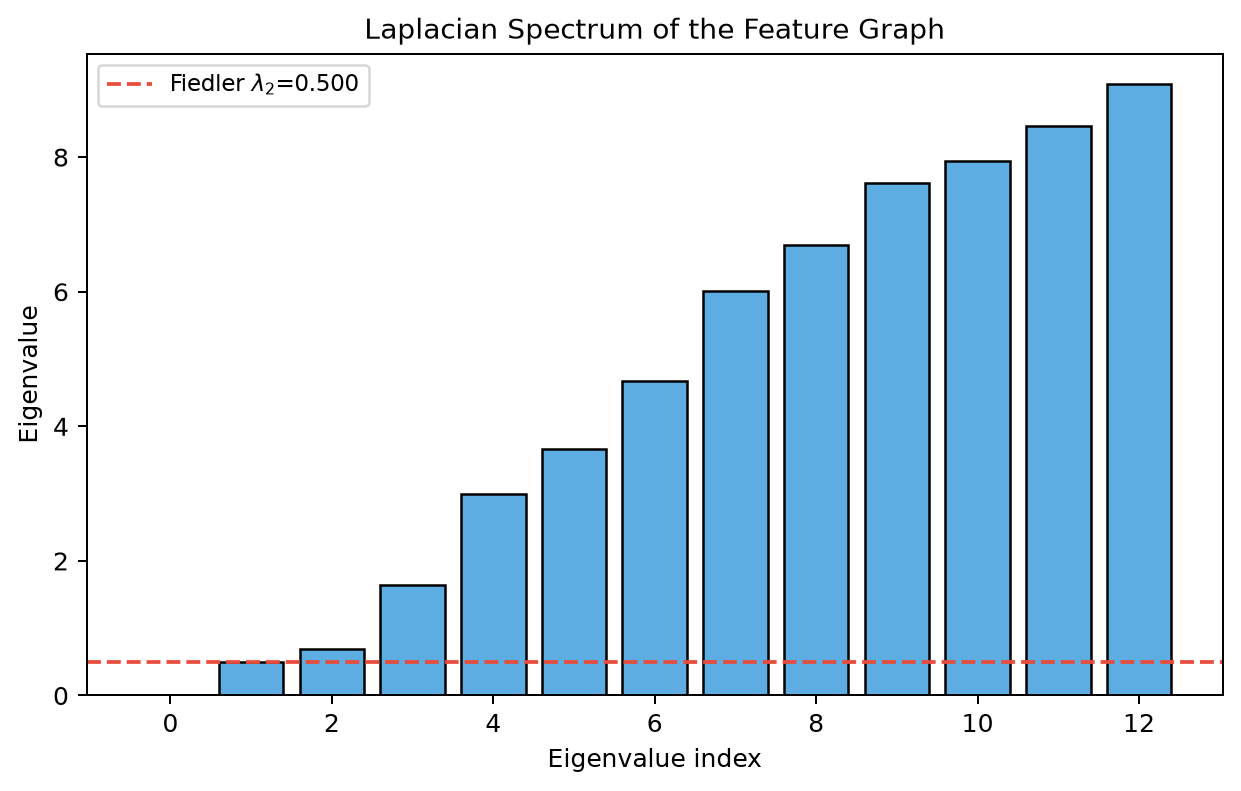
\includegraphics[width=\columnwidth]{fig05_spectral.png}
\caption{Laplacian spectrum of the $|r|$-weighted feature graph. The
positive Fiedler value $\lambda_2$ confirms a single connected component,
the structural guarantee provided by the MST augmentation.}
\label{fig:spectral}
\end{figure}

\begin{figure}[t]
\centering
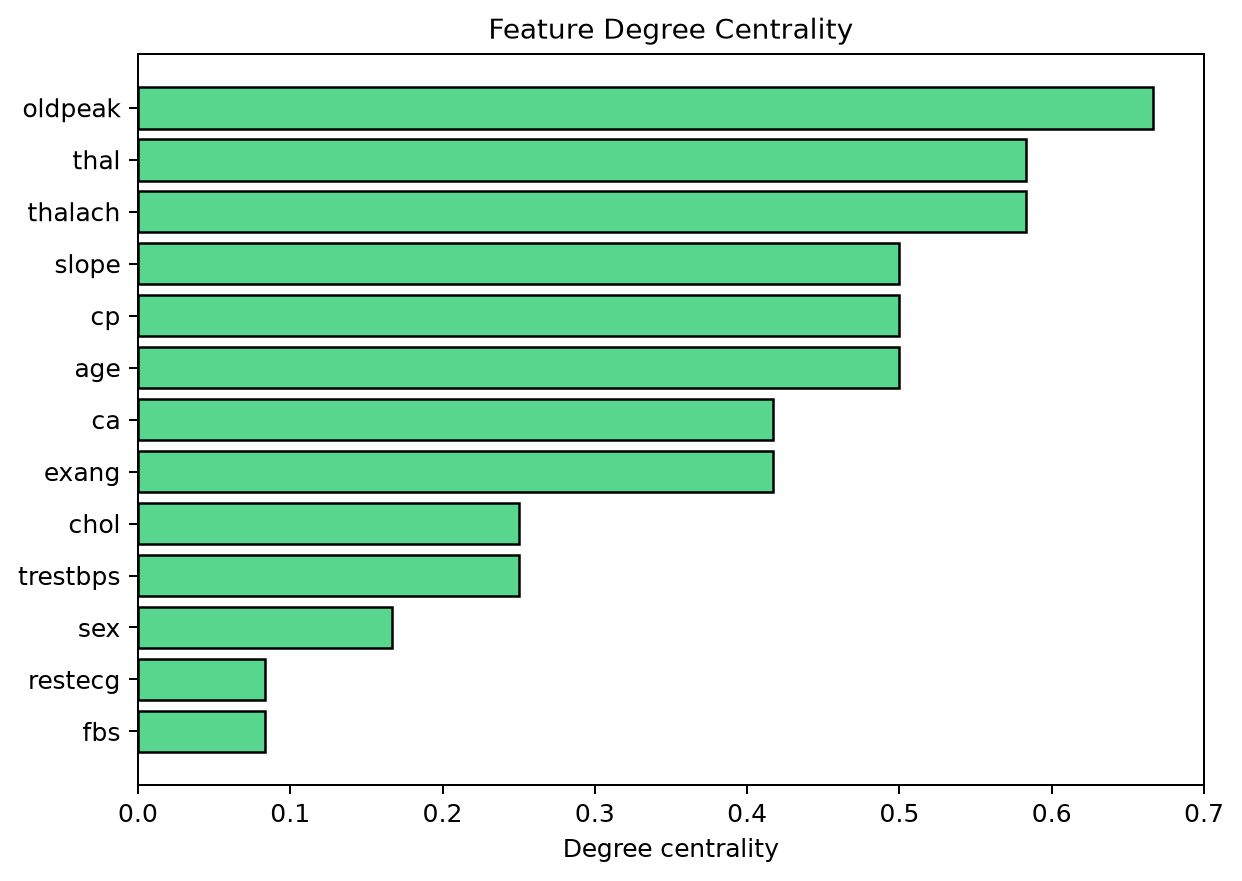
\includegraphics[width=\columnwidth]{fig06_degree_centrality.png}
\caption{Degree centrality of the feature nodes. Hub features coincide
with the highest target-correlated variables, linking graph structure to
clinical relevance.}
\label{fig:centrality}
\end{figure}


\subsection{Patient-graph encoding}
Every patient is encoded as a graph with thirteen nodes sharing the
fold's edge index; the node feature vector is the patient's scalar value
for each clinical feature, i.e.\ $x\in\mathbb{R}^{13\times1}$. Only the
node values vary across patients; the topology is common within a fold.

\section{Model}
The classifier (Fig.~\ref{fig:arch}) stacks two graph convolutional
layers~\cite{kipf2017gcn}, each followed by batch normalisation and ReLU,
with dropout between layers. A global mean-pooling readout produces a
graph-level embedding that a linear layer maps to a disease probability.
Formally, with $H^{(0)}=X$ and normalised adjacency $\hat{A}$,
\begin{equation}
H^{(l+1)}=\mathrm{ReLU}\!\left(\mathrm{BN}\!\left(\hat{A}H^{(l)}W^{(l)}\right)\right),
\end{equation}
and the prediction is
$\hat{y}=\sigma\!\left(w^\top\,\mathrm{MeanPool}(H^{(2)})+b\right)$.
Hyperparameters are listed in Table~\ref{tab:hyperparams}.

\begin{figure*}[t]
\centering

\includegraphics[width=\textwidth]{fig07_architecture.png}
\caption{Two-layer GCN architecture with batch normalisation, dropout,
global mean pooling and a sigmoid output head.}
\label{fig:arch}
\end{figure*}

% ---- begin inlined: table_hyperparameters ----
\begin{table}[t]
\centering
\caption{Training and architecture hyperparameters.}
\label{tab:hyperparams}
\small
\begin{tabular}{p{3.1cm}p{4.6cm}}
\toprule
Hyperparameter & Value \\
\midrule
Node feature dim & 1 (scalar clinical value) \\
\# Nodes & 13 (clinical features) \\
Continuous features (scaled) & 5 \\
Categorical features (raw) & 8 \\
Correlation metric & Pearson \\
Correlation threshold $\tau$ & 0.15 \\
Graph augmentation & Minimum Spanning Tree ($d = 1 - |r|$) \\
GCN layers & 2 \\
Hidden dimension & 32 \\
Normalization & BatchNorm1d \\
Activation & ReLU \\
Dropout & 0.30 \\
Readout & Global mean pooling \\
Output head & Linear(32$\to$1) + sigmoid \\
Loss & BCEWithLogits (balanced) \\
Optimizer & Adam \\
Learning rate & 1e-3 \\
Weight decay & 1e-4 \\
Gradient clipping & max-norm 1.0 \\
Batch size & 32 \\
Max epochs & 150 \\
Early stopping patience & 25 (val loss) \\
Decision threshold & tuned on inner-validation (F1) \\
Cross-validation & 5-fold Stratified \\
Inner val split & 15\% of train fold (stratified) \\
Scaling & MinMax (continuous cols), fit in-fold \\
Framework & PyTorch 2.x + PyG 2.7, CPU \\
Seeds & 42, 7, 123 \\
\bottomrule
\end{tabular}
\end{table}
%% ---- end inlined: table_hyperparameters ----

\section{Experimental Setup}
\label{sec:setup}
\subsection{Protocol}
All models are evaluated with five-fold stratified cross-validation,
repeated over three random seeds ($42,7,123$). Within each fold a
stratified $15\%$ inner-validation split is used for early stopping and
decision-threshold selection. Every preprocessing step---scaling and
graph construction---is fit on the training partition only; test folds are
never used for scaling, graph construction, model selection or threshold
tuning. Reported values are mean$\pm$standard deviation across folds and
seeds.

\subsection{Baselines}
Six classical models---Logistic Regression, Random Forest, Gradient
Boosting, a Multilayer Perceptron, XGBoost~\cite{chen2016xgboost} and
LightGBM~\cite{ke2017lightgbm}---are trained under \emph{identical}
folds with in-fold standardisation and identical inner-validation
threshold tuning, ensuring a strictly fair comparison. The two
gradient-boosted-tree models are included specifically because they are
the strongest tabular baselines in the current literature and were
absent from the original baseline suite; their inclusion tests whether a
more competitive classical model closes the accuracy-parity gap reported
in Section~\ref{sec:results}.

We additionally implement the \emph{conventional patient-similarity GNN}
as a fifth baseline, so that the two graph formulations can be compared
empirically rather than only conceptually. Nodes are patients, node
features are the patient's scaled clinical values, and edges form a
symmetric $k$-nearest-neighbour graph in feature space; the task is
transductive node classification. Depth, hidden width, dropout,
optimiser, early stopping, folds and seeds are identical to the
feature-node model. To avoid understating the baseline, $k$ is swept over
$\{5,10,15,20\}$ and the best value by ROC-AUC is retained ($k=15$). The
scaler is fit on inner-training patients only and the $k$-NN graph is
built from \emph{features alone}---never labels---with the loss masked to
training nodes; test-node labels are never observed. Test-node features
do participate in message passing, which is inherent to the transductive
formulation and is precisely the property we wish to expose.

\subsection{Metrics and statistics}
We report accuracy, precision, recall, F1, ROC-AUC, MCC~\cite{matthews1975}
and specificity. Statistical significance is assessed with McNemar's
test~\cite{mcnemar1947} on the pooled out-of-fold predictions and the
Wilcoxon signed-rank test~\cite{wilcoxon1945} on per-fold F1. Where
configurations are compared on the identical (seed $\times$ fold)
partitions, fold-level metrics are \emph{paired} and the signed-rank test
is applied to those pairs.

Wherever a family of hypotheses is tested together---several metrics,
several baselines, or several cohorts within one analysis---we control the
family-wise error rate with the Holm--Bonferroni
procedure~\cite{holm1979} and report both the raw and the adjusted
$p$-value, judging significance on the adjusted value. This policy is
applied uniformly to every significance table in the paper. It is
deliberately \emph{not} applied to the per-seed rows of
Table~\ref{tab:formstats}, whose rows are replicates of a single
hypothesis rather than distinct hypotheses; correcting across replicates
would inflate the $p$-value of one test rather than control a family.

\subsection{Reproducibility}
\label{sec:repro}
Experiments use Python~3.13, PyTorch~2.x~\cite{paszke2019pytorch},
PyTorch~Geometric~2.7~\cite{fey2019pyg} and scikit-learn~1.7~\cite{pedregosa2011scikit}
on CPU. Random seeds are fixed for NumPy, Python and PyTorch, and
per-fold weight initialisation is seeded for determinism. The model has $1{,}281$ parameters; wall-clock training time and peak
memory are reported with the released code.

\textbf{Data and code availability.} The UCI Cleveland, Hungarian,
Switzerland and Long-Beach-VA heart-disease cohorts are publicly
available from the UCI Machine Learning
Repository~\cite{uci_heart,detrano1989}. All experiment code, fixed
seeds, generated result tables and figure-producing scripts are released
at
%% SUBMISSION-TODO: replace with the public repository (or archived DOI).
\url{https://github.com/USERNAME/REPOSITORY}.
Every table and figure in this paper is regenerated end-to-end by that
code; no result is transcribed by hand.

\section{Results and Discussion}
\label{sec:results}
\subsection{Predictive performance}
Table~\ref{tab:comparison} reports the main comparison, which includes
gradient-boosted-tree baselines (XGBoost, LightGBM) in addition to
Logistic Regression, Random Forest and an MLP, all under the identical
5-fold $\times$ 3-seed protocol with in-fold scaling and inner-validation
threshold tuning. The feature-node GCN attains the highest mean ROC-AUC
(0.906) and specificity (0.824) among all seven models; Logistic
Regression is marginally ahead on accuracy (0.818 vs.\ 0.813), F1 (0.810
vs.\ 0.799) and MCC (0.646 vs.\ 0.632), and Random Forest is comparable
on ROC-AUC (0.904) but trails on the remaining metrics. The two
boosted-tree baselines do not close the gap either: XGBoost reaches
ROC-AUC $0.885\pm0.033$ and LightGBM $0.882\pm0.036$, both below every
one of the three leading models on this metric, though still within a
comparable range on accuracy and F1. All differences among the leading
models are within one standard deviation of each other.
Pooled out-of-fold point metrics, which aggregate every held-out
prediction into a single estimate rather than averaging fold-wise, are
reported in Table~\ref{tab:pooled}. They agree closely with the
fold-averaged values on the ranking metrics (ROC-AUC differs by at most
$0.005$ for every model), while threshold-dependent metrics differ more
for the tree ensembles (up to $0.053$ on specificity for Random Forest
and $0.052$ on MCC for LightGBM), as expected when a single pooled
threshold replaces per-fold tuning. The ordering of models is unchanged.
The pooled out-of-fold ROC and precision--recall
curves (Fig.~\ref{fig:rocpr}) confirm that all models operate in a
high-AUC regime ($\approx 0.90$), which is expected on a small,
near-balanced cohort and implies limited head-room for any single model.
The GCN's errors are balanced across types,
and its predicted-probability distribution is well separated by class
(Fig.~\ref{fig:calib}, right). The calibration curve
(Fig.~\ref{fig:calib}, left) indicates reasonable probability calibration
after inner-validation threshold tuning.

% ---- begin inlined: combined_performance ----
\begin{table*}[t]
\centering
\caption{Predictive performance under the identical five-fold protocol. Panel (a) reports the fold-wise mean $\pm$ standard deviation; panel (b) reports pooled out-of-fold point estimates over all 303 patients.}
\label{tab:comparison}
\label{tab:pooled}
\footnotesize
\textbf{(a) Fold-wise mean $\pm$ std}\\[2pt]
\resizebox{\textwidth}{!}{%
\begin{tabular}{lrrrrrr}
\toprule
Model & Accuracy & Recall & F1 & ROC-AUC & MCC & Specificity \\
\midrule
GCN (Ours) & 0.8131 $\pm$ 0.0638 & 0.8011 $\pm$ 0.0748 & 0.7988 $\pm$ 0.0595 & 0.9056 $\pm$ 0.0408 & 0.6320 $\pm$ 0.1218 & 0.8237 $\pm$ 0.1170 \\
Logistic Regression & 0.8184 $\pm$ 0.0524 & 0.8444 $\pm$ 0.0842 & 0.8100 $\pm$ 0.0537 & 0.9025 $\pm$ 0.0385 & 0.6457 $\pm$ 0.1003 & 0.7971 $\pm$ 0.0940 \\
Random Forest & 0.7921 $\pm$ 0.0558 & 0.8393 $\pm$ 0.0844 & 0.7893 $\pm$ 0.0432 & 0.9044 $\pm$ 0.0336 & 0.6035 $\pm$ 0.0933 & 0.7524 $\pm$ 0.1421 \\
Gradient Boosting & 0.7823 $\pm$ 0.0496 & 0.8026 $\pm$ 0.0758 & 0.7716 $\pm$ 0.0502 & 0.8721 $\pm$ 0.0390 & 0.5708 $\pm$ 0.0945 & 0.7648 $\pm$ 0.0921 \\
MLP & 0.7822 $\pm$ 0.0480 & 0.8227 $\pm$ 0.0643 & 0.7764 $\pm$ 0.0450 & 0.8680 $\pm$ 0.0320 & 0.5728 $\pm$ 0.0914 & 0.7482 $\pm$ 0.0849 \\
XGBoost & 0.7944 $\pm$ 0.0459 & 0.8515 $\pm$ 0.0677 & 0.7924 $\pm$ 0.0386 & 0.8845 $\pm$ 0.0332 & 0.6027 $\pm$ 0.0831 & 0.7463 $\pm$ 0.0981 \\
LightGBM & 0.7922 $\pm$ 0.0456 & 0.7914 $\pm$ 0.0633 & 0.7772 $\pm$ 0.0493 & 0.8817 $\pm$ 0.0355 & 0.5844 $\pm$ 0.0919 & 0.7929 $\pm$ 0.0527 \\
\bottomrule
\end{tabular}
}
\vspace{7pt}
\textbf{(b) Pooled out-of-fold point estimates}\\[2pt]
\begin{tabular}{lrrrrrr}
\toprule
Model & Accuracy & Recall & F1 & ROC-AUC & MCC & Specificity \\
\midrule
GCN (Ours) & 0.8053 & 0.7986 & 0.79 & 0.9034 & 0.6087 & 0.811 \\
Logistic Regression & 0.8152 & 0.8417 & 0.8069 & 0.9062 & 0.6322 & 0.7927 \\
Random Forest & 0.8152 & 0.8273 & 0.8042 & 0.907 & 0.6303 & 0.8049 \\
Gradient Boosting & 0.7921 & 0.8201 & 0.7835 & 0.8759 & 0.5864 & 0.7683 \\
MLP & 0.7921 & 0.8273 & 0.785 & 0.8639 & 0.5876 & 0.7622 \\
XGBoost & 0.802 & 0.8129 & 0.7902 & 0.8825 & 0.6038 & 0.7927 \\
LightGBM & 0.8185 & 0.8273 & 0.807 & 0.8869 & 0.6366 & 0.811 \\
\bottomrule
\end{tabular}
\end{table*}
%% ---- end inlined: combined_performance ----


\begin{figure*}[t]
\centering
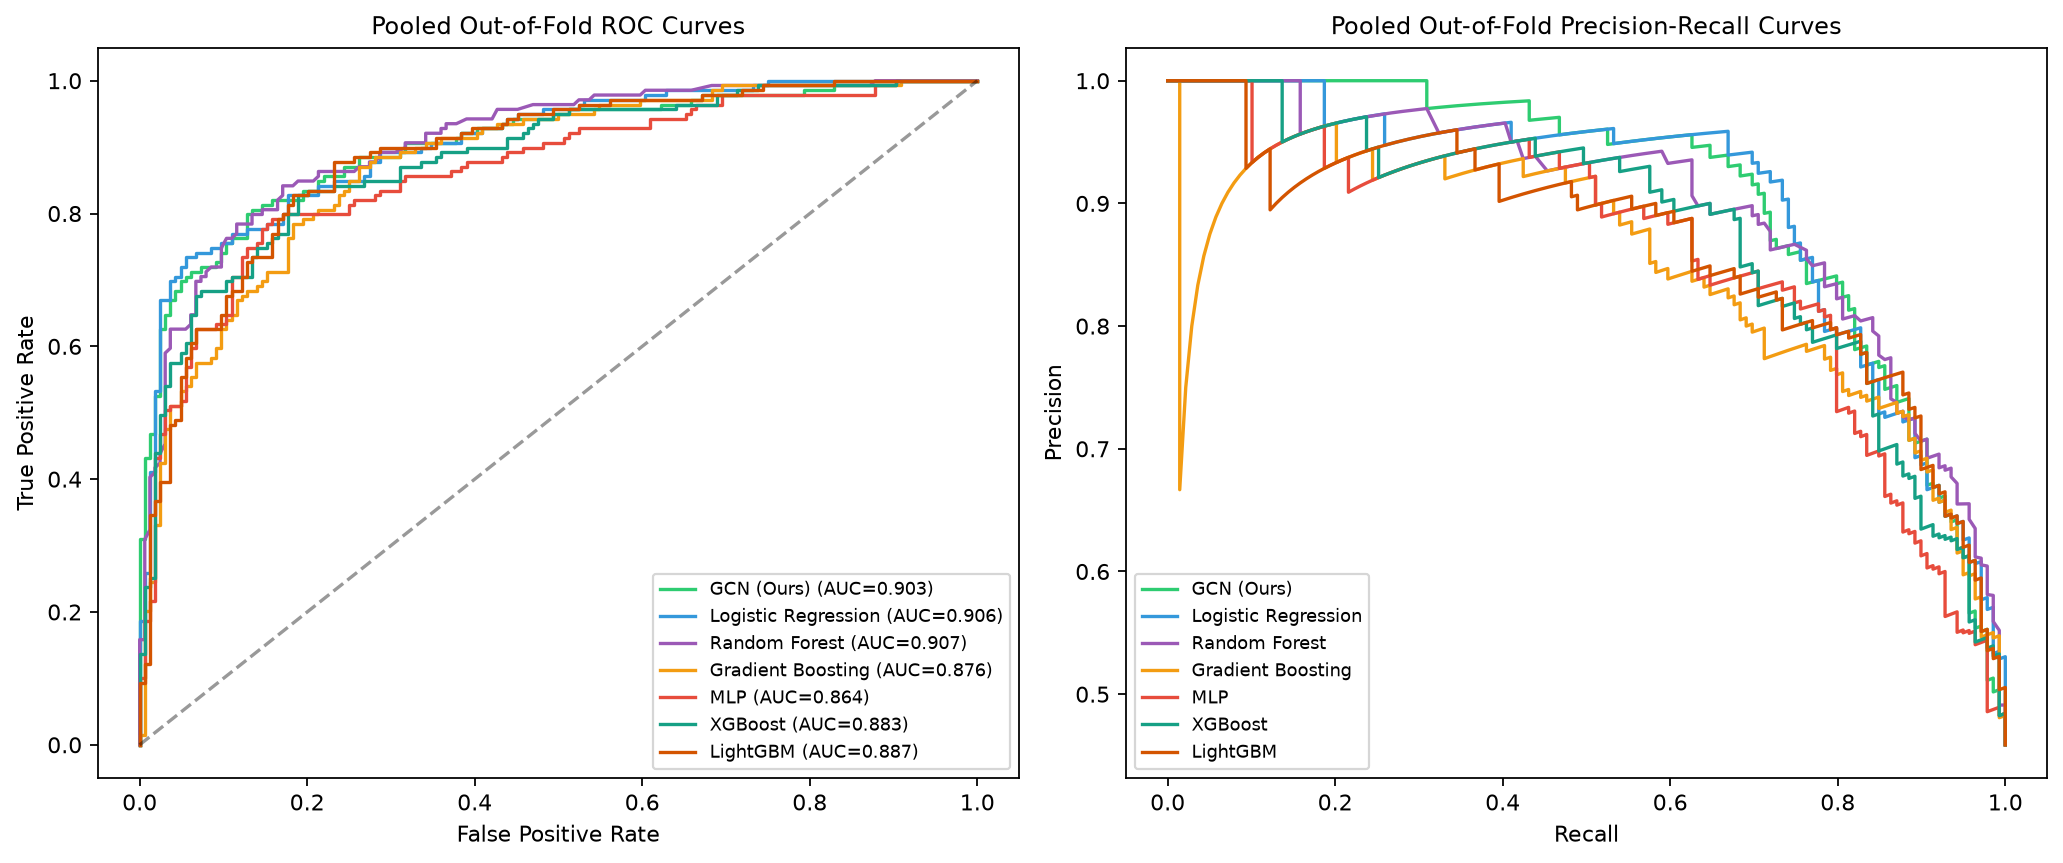
\includegraphics[width=\textwidth]{fig10_roc_pr.png}
\caption{Pooled out-of-fold ROC (left) and precision--recall (right)
curves. All models achieve comparable, high AUC, underscoring the
performance ceiling of the cohort.}
\label{fig:rocpr}
\end{figure*}


\begin{figure*}[t]
\centering
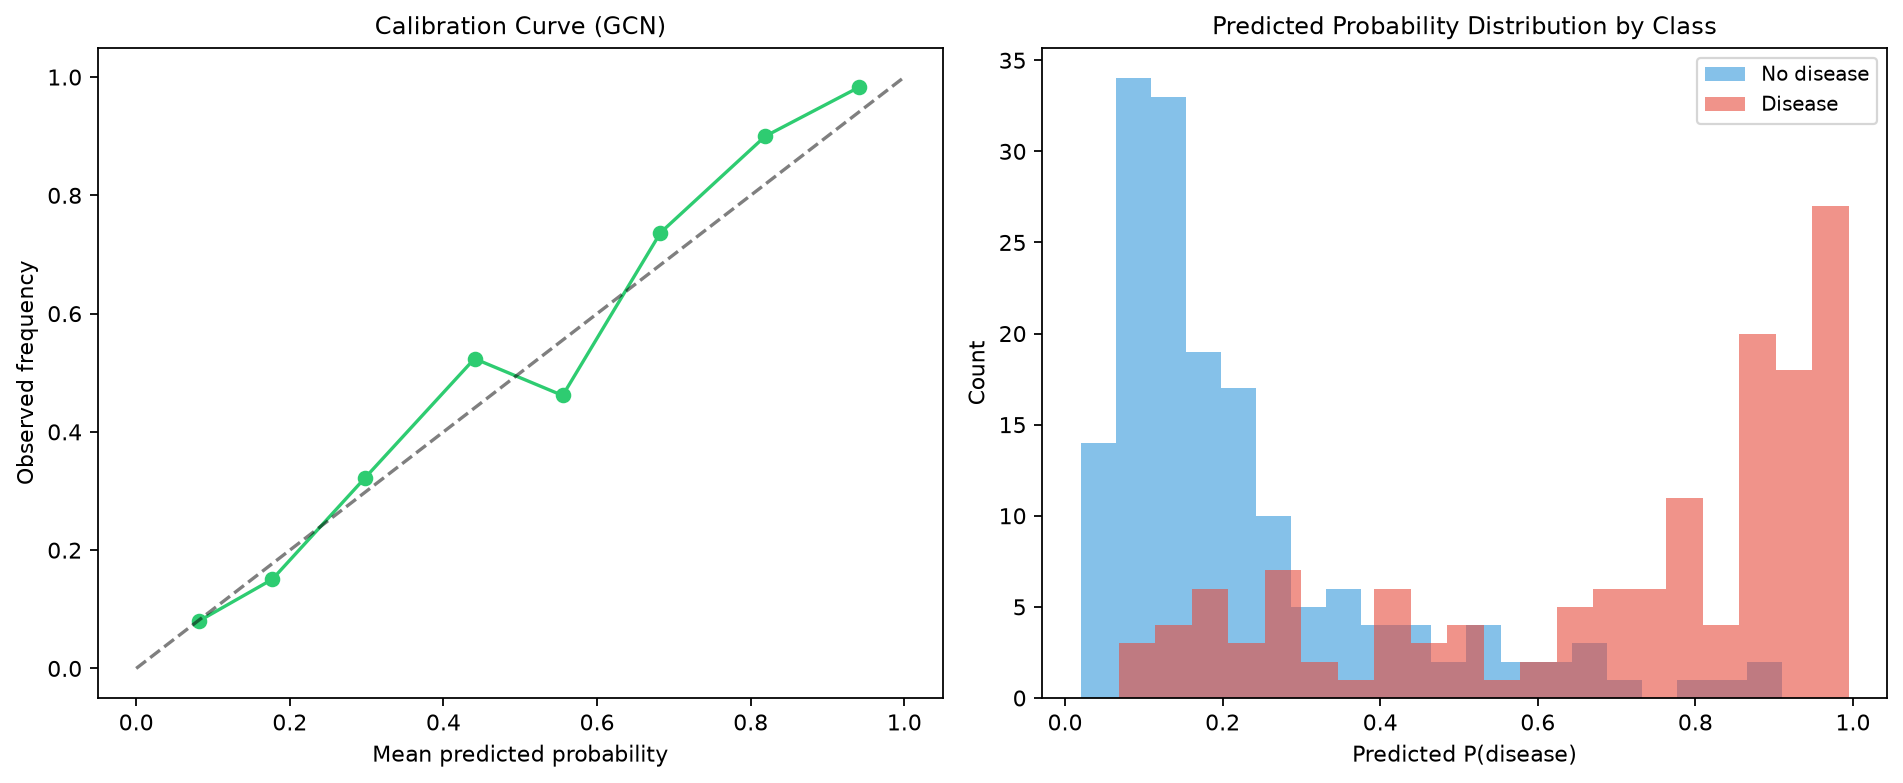
\includegraphics[width=\textwidth]{fig28_calibration_probdist.png}
\caption{Left: reliability (calibration) curve for the GCN. Right:
distribution of predicted disease probabilities by true class,
demonstrating clear separation.}
\label{fig:calib}
\end{figure*}

\subsection{Statistical significance}
Table~\ref{tab:stats} reports the significance tests against
\emph{every} baseline in Table~\ref{tab:comparison}, not a subset: the
two linear/ensemble baselines (Logistic Regression, Random Forest), the
three gradient-boosting baselines (Gradient Boosting, LightGBM,
XGBoost) and the neural baseline (MLP). None of the twelve tests (six
comparisons $\times$ two test types) approaches the $0.05$ significance
level after Holm correction across the family: McNemar's test on the
pooled out-of-fold predictions gives $p=0.70$ against Logistic
Regression, $p=0.77$ against Random Forest, $p=0.68$ against Gradient
Boosting, $p=0.68$ against MLP, $p=1.00$ against XGBoost and $p=0.66$
against LightGBM, and the Wilcoxon signed-rank test on per-fold F1 gives
$p=0.25$, $p=0.51$, $p=0.11$, $p=0.09$, $p=0.60$ and $p=0.15$,
respectively (Holm-adjusted $p\geq0.57$ throughout). We therefore
characterise the GCN as \emph{statistically indistinguishable from}
strong classical baselines---including modern gradient-boosted trees and
a comparably-sized MLP---not as a decisive improvement. This honest
positioning is, in our view, more credible than an inflated accuracy
claim and redirects the contribution toward representation and
interpretability.

% ---- begin inlined: table_statistical_tests ----
\begin{table*}[t]
\centering
\caption{Statistical significance of the GCN vs. baseline classifiers (McNemar on pooled OOF predictions; Wilcoxon signed-rank on per-fold F1).}
\label{tab:stats}
\footnotesize
\resizebox{\textwidth}{!}{%
\begin{tabular}{lrrrrrrrrr}
\toprule
Comparison & $b$ & $c$ & McNemar stat & McNemar $p$ & Wilcoxon $p$ & Holm p (McNemar) & Sig. Holm (McNemar) & Holm p (Wilcoxon(foldF1)) & Sig. Holm (Wilcoxon(foldF1)) \\
\midrule
GCN vs Logistic Regression & 15 & 12 & 0.1481 & 0.7003 & 0.2455 & 1.0 & no & 0.7365 & no \\
GCN vs Random Forest & 24 & 21 & 0.0889 & 0.7656 & 0.5098 & 1.0 & no & 1.0 & no \\
GCN vs Gradient Boosting & 25 & 29 & 0.1667 & 0.6831 & 0.107 & 1.0 & no & 0.5676 & no \\
GCN vs MLP & 24 & 28 & 0.1731 & 0.6774 & 0.0946 & 1.0 & no & 0.5676 & no \\
GCN vs XGBoost & 25 & 26 & 0.0 & 1.0 & 0.5995 & 1.0 & no & 1.0 & no \\
GCN vs LightGBM & 25 & 21 & 0.1957 & 0.6583 & 0.1514 & 1.0 & no & 0.6056 & no \\
\bottomrule
\end{tabular}
}
\end{table*}
%% ---- end inlined: table_statistical_tests ----

\subsection{Comparison with the patient-similarity formulation}
\label{sec:formulation}
The premise of this work is that a feature-node graph is a more suitable
inductive bias for clinical tabular data than the conventional
patient-similarity graph. We test that premise directly.

A $k$-sweep of the patient-similarity baseline identifies $k=15$ as its
own best setting, which is used throughout.
Table~\ref{tab:formulation} compares the two formulations under the
identical protocol. The feature-node model is ahead on every metric---most
clearly on ROC-AUC ($0.905\pm0.041$ versus $0.889\pm0.036$)---but the
margin is modest. Per-seed DeLong tests~\cite{delong1988} on the pooled out-of-fold
predictions (Table~\ref{tab:formstats}) give $p=0.351$, $0.910$ and
$0.017$: the direction is consistent across all three seeds, yet the
difference reaches significance in only one. \emph{In distribution we
therefore claim parity with a consistent directional advantage, not a
demonstrated win.}

The more informative difference is structural. The patient-similarity
model is transductive: before it can score any patient it requires a
cohort-level graph, so it cannot classify an isolated individual. The
feature-node model is inductive---each patient is an independent
graph---and the topology learned on the development cohort transfers
directly. Section~\ref{sec:external} shows that this distinction has
practical consequences under distribution shift.

% ---- begin inlined: combined_patient ----
\begin{table*}[t]
\centering
\caption{Feature-node versus patient-similarity formulation in distribution. Panel (a) reports the paired comparison; panel (b) reports the significance tests.}
\label{tab:formulation}
\label{tab:formstats}
\footnotesize
\textbf{(a) Paired comparison}\\[2pt]
\resizebox{\textwidth}{!}{%
\begin{tabular}{lrrrrrrr}
\toprule
Formulation & Accuracy & Precision & Recall & F1 & ROC-AUC & MCC & Specificity \\
\midrule
Feature-node graph (Ours) & 0.8109 $\pm$ 0.0652 & 0.8044 $\pm$ 0.0999 & 0.8011 $\pm$ 0.0748 & 0.7971 $\pm$ 0.0597 & 0.9051 $\pm$ 0.0413 & 0.6280 $\pm$ 0.1240 & 0.8196 $\pm$ 0.1208 \\
Patient-similarity graph (k=15) & 0.8021 $\pm$ 0.0467 & 0.7791 $\pm$ 0.0963 & 0.8275 $\pm$ 0.0970 & 0.7931 $\pm$ 0.0447 & 0.8891 $\pm$ 0.0358 & 0.6184 $\pm$ 0.0895 & 0.7807 $\pm$ 0.1163 \\
\bottomrule
\end{tabular}
}
\vspace{7pt}
\textbf{(b) Significance tests}\\[2pt]
\begin{tabular}{lrrrrrrr}
\toprule
Seed & AUC (feature-node) & AUC (patient-sim) & $\Delta$AUC & b & c & McNemar p & DeLong p \\
\midrule
42.0 & 0.9033 & 0.8909 & 0.0124 & 22.0 & 21.0 & 1.0 & 0.3506 \\
7.0 & 0.8915 & 0.8903 & 0.0012 & 20.0 & 17.0 & 0.7423 & 0.9097 \\
123.0 & 0.9005 & 0.8726 & 0.0279 & 11.0 & 23.0 & 0.0592 & 0.01708 \\
\bottomrule
\end{tabular}
\end{table*}
%% ---- end inlined: combined_patient ----

\subsection{Deployment characteristics}
\label{sec:deploy}
Because deployability is one of the three properties on which we rest the
case for this formulation (\textbf{P2}), we measure it rather than assert
it (Table~\ref{tab:deploy}).

\textbf{Inductive single-patient inference.} We scored held-out patients
strictly one at a time, constructing each patient's graph in isolation
with no other patient present, and compared the result against batch
scoring. The maximum absolute deviation over all patients was
$3.0\times10^{-8}$, i.e.\ numerically identical: the model's output for a
patient does not depend on which other patients are present. Mean latency
was $2.56$\,ms per patient (median $2.43$\,ms, p95 $2.93$\,ms) on CPU. The
patient-similarity baseline of Section~\ref{sec:formulation} admits no
analogous measurement, because it cannot produce a prediction for an
isolated patient at all.

\textbf{Footprint.} The deployed model has $1{,}281$ trainable parameters
and serialises to $11.4$\,KB; training completes in seconds and peak
memory stays below $2$\,MB. Nothing in the
pipeline requires a GPU.

\textbf{Calibration.} Discrimination is not sufficient for a decision
aid: predicted risks must also be calibrated. Table~\ref{tab:calib}
reports Brier score~\cite{brier1950} and expected calibration error
(ECE)~\cite{naeini2015ece}. Out-of-fold on
Cleveland the GCN is the best-calibrated of the three models
(Brier $0.124$, ECE $0.042$, against $0.124/0.047$ for Logistic
Regression and $0.126/0.055$ for Random Forest). The more interesting
behaviour appears under transport. Logistic Regression's calibration
collapses on every external cohort (ECE $0.318$, $0.530$, $0.471$),
whereas the GCN degrades far more gracefully on Hungarian
(ECE $0.091$ versus $0.318$ and $0.209$)---a $3.5\times$ advantage over
the linear baseline---and remains competitive with Random Forest on VA
($0.195$ versus $0.169$). On Switzerland, whose disease prevalence is
$93\%$, all three models are poorly calibrated and Random Forest is the
least bad ($0.356$ versus $0.453$). Retaining calibration under
distribution shift, not merely ranking ability, is in our view the most
practically relevant transport result in this paper.

\textbf{Clinical utility, and where it is absent.} Calibration and
discrimination still do not establish that a model is worth using. We
therefore computed decision curves~\cite{vickers2006dca}, reporting net
benefit
$\mathrm{NB}=\mathrm{TP}/n-(\mathrm{FP}/n)\,p_t/(1-p_t)$ across
clinically plausible risk thresholds against the default strategy of
treating every patient.

The outcome divides cleanly by cohort prevalence, and we report it
without selection. On Hungarian, whose $36\%$ prevalence is clinically
realistic, the GCN yields the highest net benefit at every threshold
examined and exceeds treat-all by a widening margin as $p_t$ grows
($0.220$ versus $0.085$ at $p_t=0.30$; $0.164$ versus $-0.281$ at
$p_t=0.50$). On Switzerland ($93\%$ prevalence) and VA ($79\%$), by
contrast, \emph{no} model improves on treating everyone: at $p_t=0.30$
the GCN attains $0.687$ against treat-all's $0.902$ on Switzerland, and
$0.631$ against $0.694$ on VA. We regard this as a property of those
cohorts rather than of the model---when nearly every patient is diseased,
the treat-all strategy is close to optimal by construction and any
selective rule can only forgo true positives. It nevertheless bounds the
claim we are entitled to make: \emph{demonstrated clinical utility rests
on the single external cohort with a realistic prevalence}, and
prospective evaluation in a screening population remains necessary.

% ---- begin inlined: table_deployment ----
\begin{table}[t]
\centering
\caption{Deployment characteristics of the feature-node model. Inference is inductive: patients are scored individually with no cohort present.}
\label{tab:deploy}
\small
\begin{tabular}{p{3.1cm}p{4.6cm}}
\toprule
Property & Value \\
\midrule
Scores an isolated patient & Yes (inductive) \\
Cohort graph required at inference & No \\
Patients scored individually & 46 \\
Max deviation vs batch scoring & 2.98e-08 \\
Latency per patient, mean & 2.564 ms \\
Latency per patient, median & 2.430 ms \\
Latency per patient, p95 & 2.933 ms \\
Trainable parameters & 1,281 \\
Serialised model size & 11.4 KB \\
Hardware & CPU only \\
\bottomrule
\end{tabular}
\end{table}
%% ---- end inlined: table_deployment ----
% ---- begin inlined: table_calibration ----
\begin{table*}[t]
\centering
\caption{Calibration of predicted risks. Brier score and expected calibration error (ECE, 10 bins), out-of-fold on Cleveland and on each external cohort. Lower is better.}
\label{tab:calib}
\footnotesize
\begin{tabular}{lrrr}
\toprule
Setting & Model & Brier & ECE \\
\midrule
Cleveland (OOF) & GCN (Ours) & 0.1238 $\pm$ 0.0023 & 0.0421 $\pm$ 0.0090 \\
Cleveland (OOF) & Logistic Regression & 0.1243 $\pm$ 0.0033 & 0.0467 $\pm$ 0.0031 \\
Cleveland (OOF) & Random Forest & 0.1262 $\pm$ 0.0014 & 0.0546 $\pm$ 0.0061 \\
Hungarian & GCN (Ours) & 0.1416 $\pm$ 0.0059 & 0.0907 $\pm$ 0.0105 \\
Hungarian & Logistic Regression & 0.3153 $\pm$ 0.0116 & 0.3181 $\pm$ 0.0136 \\
Hungarian & Random Forest & 0.1969 $\pm$ 0.0069 & 0.2086 $\pm$ 0.0030 \\
Switzerland & GCN (Ours) & 0.2975 $\pm$ 0.0343 & 0.4526 $\pm$ 0.0340 \\
Switzerland & Logistic Regression & 0.5279 $\pm$ 0.2047 & 0.5301 $\pm$ 0.2056 \\
Switzerland & Random Forest & 0.1944 $\pm$ 0.0182 & 0.3560 $\pm$ 0.0220 \\
VA Long Beach & GCN (Ours) & 0.2054 $\pm$ 0.0085 & 0.1952 $\pm$ 0.0115 \\
VA Long Beach & Logistic Regression & 0.4686 $\pm$ 0.1730 & 0.4709 $\pm$ 0.1728 \\
VA Long Beach & Random Forest & 0.1857 $\pm$ 0.0021 & 0.1693 $\pm$ 0.0120 \\
\bottomrule
\end{tabular}
\end{table*}
%% ---- end inlined: table_calibration ----

\subsection{Learned representation}
Training is stable under early stopping, and
Fig.~\ref{fig:embed} projects the learned graph-level embeddings with PCA
and t-SNE. Disease and non-disease patients form largely separated
clusters, indicating that the pooled representation captures
class-discriminative structure despite the one-dimensional node features.


\begin{figure*}[t]
\centering
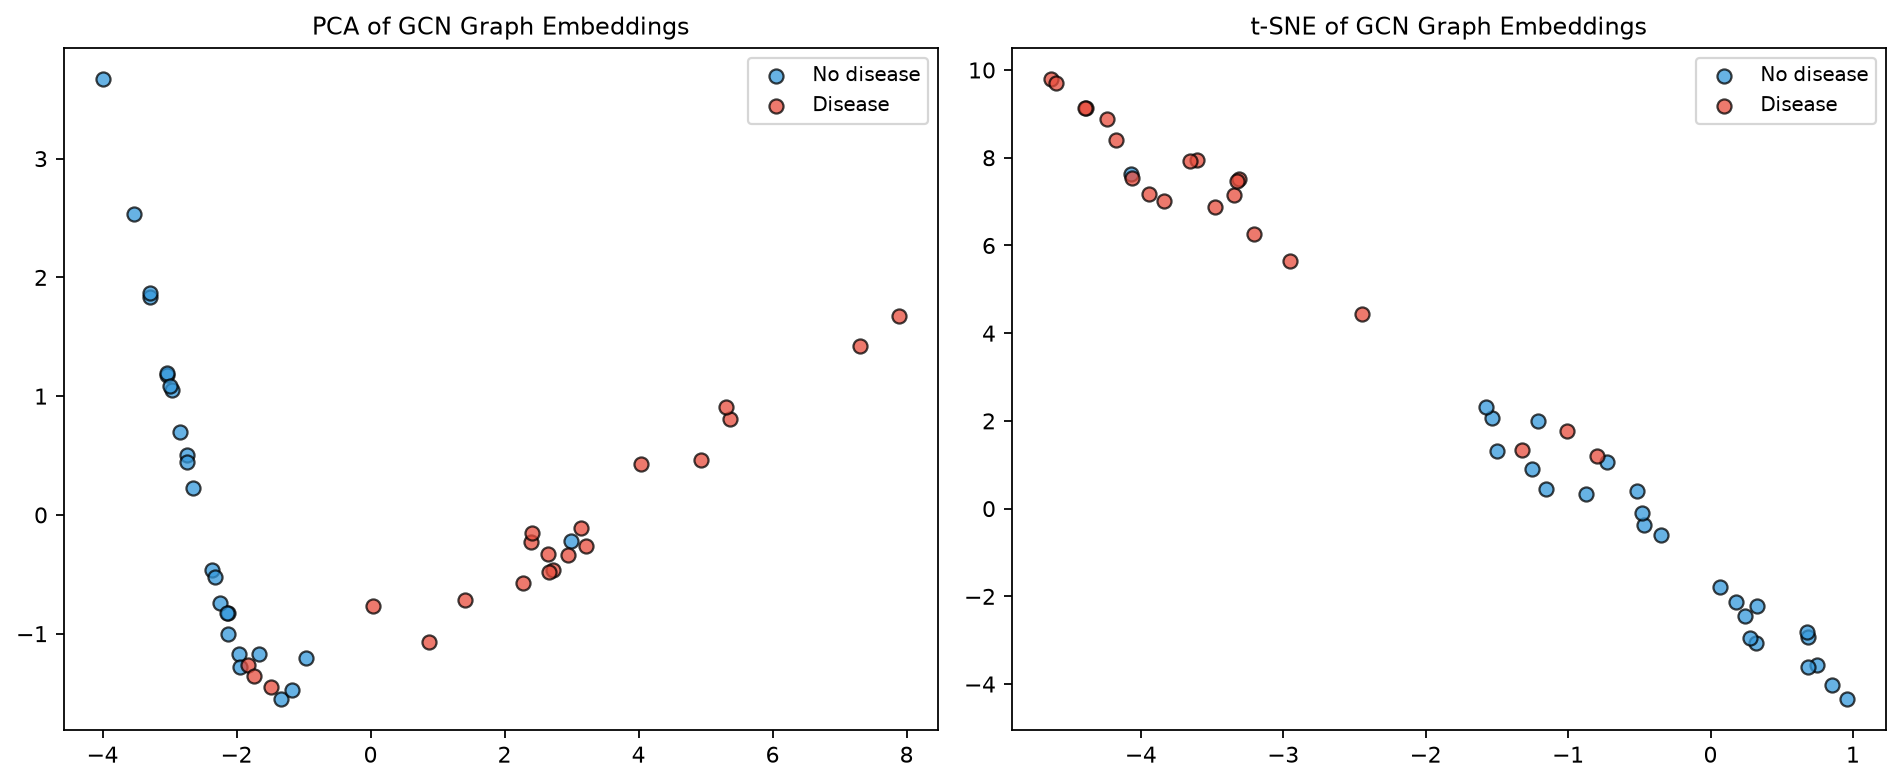
\includegraphics[width=\textwidth]{fig19_embeddings.png}
\caption{PCA (left) and t-SNE (right) projections of the learned
graph-level embeddings on the held-out test set. The two classes form
largely separated clusters.}
\label{fig:embed}
\end{figure*}

\subsection{Ablation study}
\label{sec:ablation}
Table~\ref{tab:ablation} presents the complete ablation; panel~(b)
isolates the effect of each design choice. Four
findings emerge.

\emph{(i) Selective sparsity helps.} The fully connected graph is the
weakest configuration (Table~\ref{tab:ablation}), confirming that
indiscriminate connectivity injects noise and that a sparse,
correlation-driven topology is preferable. This is the result that most
directly justifies the graph-construction contribution.

\emph{(ii) The MST aids connectivity, not accuracy.} Removing the MST
bridges leaves predictive performance essentially unchanged. This row
must be read with care, however: at $\tau=0.15$ the thresholded graph is
already connected in every fold, so the MST adds no edges and the two
conditions are in fact the \emph{same graph}
(Table~\ref{tab:mstactivation}); the residual difference is
run-to-run non-determinism rather than a component effect. The
augmentation is tested properly in Section~\ref{sec:graph} at
$\tau=0.20$, where it is active: there it restores a single connected
component in $5/5$ folds without changing any metric significantly. We
therefore present the MST as a \emph{structural} guarantee---validated by
the positive Fiedler value of Fig.~\ref{fig:spectral}---rather than as a
source of \emph{internal} accuracy gains. This ablation, like every other
row in this table, is computed within the development cohort and is by
construction blind to any effect that appears only under distribution
shift; Section~\ref{sec:tauregime} examines the same topologies on
external cohorts and finds an ordering that this table cannot see.

\emph{(iii) Message passing and correlation structure give small,
consistent benefits.} The correlation graph modestly outperforms an
edge-count-matched random graph and the no-edge (independent-node)
baseline, indicating that the specific feature-interaction topology, and
not merely the presence of edges, carries useful signal.

\emph{(iv) Two layers are preferable to one}, while the model is robust to
readout choice, dropout and hidden width within one standard deviation
(Table~\ref{tab:ablation}); this
robustness is desirable
for deployment because it reduces sensitivity to hyperparameter choices.

\emph{(v) The choice of message-passing operator is not critical.}
Because a natural objection to a GCN is that attention-based or more
expressive operators might do better, we repeat the entire protocol with
GAT, GraphSAGE and GIN substituted for GCNConv, holding graph
construction, depth, width, readout, folds and seeds fixed
(Table~S2, Supplementary Material). No operator differs significantly from GCN:
DeLong $p\ge0.63$ and McNemar $p\ge0.057$ in every comparison
(Table~S2). GIN attains a nominally higher accuracy
($0.824$ versus $0.811$), F1 and MCC, but the \emph{lowest} ROC-AUC of
the four and requires $2.6\times$ the parameters ($3{,}393$ versus
$1{,}281$); GAT and GraphSAGE fall between. On a thirteen-node feature
graph the neighbourhood structure is evidently too limited for attention
or sum-aggregation to exploit. We therefore retain GCN on grounds of
\emph{parsimony}---it is the smallest model, attains the highest ROC-AUC,
and is statistically indistinguishable from more expressive
alternatives---rather than on grounds of superiority.

% ---- begin inlined: combined_ablation ----
\begin{table*}[t]
\centering
\caption{Ablation study. Panel (a) reports absolute performance for each variant, pooled over 3 seeds $\times$ 5 folds; panel (b) reports the change relative to the full model.}
\label{tab:ablation}
\label{tab:ablation_delta}
\footnotesize
\textbf{(a) Absolute performance}\\[2pt]
\resizebox{\textwidth}{!}{%
\begin{tabular}{lrrrrrr}
\toprule
Experiment & Accuracy & F1 & ROC-AUC & MCC & Recall & Specificity \\
\midrule
Full (Corr+MST) & 0.8109 $\pm$ 0.0652 & 0.7971 $\pm$ 0.0597 & 0.9051 $\pm$ 0.0413 & 0.6280 $\pm$ 0.1240 & 0.8011 $\pm$ 0.0748 & 0.8196 $\pm$ 0.1208 \\
w/o MST (Corr only) & 0.8032 $\pm$ 0.0787 & 0.7936 $\pm$ 0.0692 & 0.9027 $\pm$ 0.0437 & 0.6164 $\pm$ 0.1468 & 0.8105 $\pm$ 0.0825 & 0.7974 $\pm$ 0.1464 \\
Random graph & 0.7955 $\pm$ 0.0614 & 0.7896 $\pm$ 0.0545 & 0.8959 $\pm$ 0.0414 & 0.6056 $\pm$ 0.1115 & 0.8300 $\pm$ 0.0892 & 0.7669 $\pm$ 0.1303 \\
Fully connected & 0.8021 $\pm$ 0.0753 & 0.7920 $\pm$ 0.0729 & 0.8973 $\pm$ 0.0432 & 0.6107 $\pm$ 0.1428 & 0.8153 $\pm$ 0.0869 & 0.7911 $\pm$ 0.1208 \\
No graph (indep. nodes) & 0.8086 $\pm$ 0.0661 & 0.7916 $\pm$ 0.0685 & 0.8966 $\pm$ 0.0485 & 0.6262 $\pm$ 0.1276 & 0.7942 $\pm$ 0.1073 & 0.8214 $\pm$ 0.1191 \\
1 GCN layer & 0.8064 $\pm$ 0.0606 & 0.7906 $\pm$ 0.0628 & 0.9005 $\pm$ 0.0423 & 0.6187 $\pm$ 0.1195 & 0.7963 $\pm$ 0.0916 & 0.8155 $\pm$ 0.1052 \\
Max pooling & 0.8032 $\pm$ 0.0778 & 0.7979 $\pm$ 0.0687 & 0.8940 $\pm$ 0.0518 & 0.6179 $\pm$ 0.1427 & 0.8347 $\pm$ 0.0827 & 0.7770 $\pm$ 0.1389 \\
Add pooling & 0.8042 $\pm$ 0.0644 & 0.7936 $\pm$ 0.0566 & 0.9008 $\pm$ 0.0361 & 0.6200 $\pm$ 0.1198 & 0.8132 $\pm$ 0.0900 & 0.7973 $\pm$ 0.1331 \\
Dropout 0.0 & 0.8218 $\pm$ 0.0612 & 0.8038 $\pm$ 0.0586 & 0.9040 $\pm$ 0.0410 & 0.6473 $\pm$ 0.1189 & 0.7914 $\pm$ 0.0762 & 0.8480 $\pm$ 0.1037 \\
Dropout 0.5 & 0.8130 $\pm$ 0.0641 & 0.7988 $\pm$ 0.0599 & 0.9061 $\pm$ 0.0408 & 0.6319 $\pm$ 0.1223 & 0.8011 $\pm$ 0.0748 & 0.8237 $\pm$ 0.1170 \\
Hidden 16 & 0.7660 $\pm$ 0.1328 & 0.7752 $\pm$ 0.0773 & 0.7993 $\pm$ 0.2716 & 0.5491 $\pm$ 0.2413 & 0.8250 $\pm$ 0.1046 & 0.7166 $\pm$ 0.3005 \\
Hidden 64 & 0.8163 $\pm$ 0.0587 & 0.8009 $\pm$ 0.0586 & 0.9040 $\pm$ 0.0414 & 0.6355 $\pm$ 0.1136 & 0.8034 $\pm$ 0.0782 & 0.8272 $\pm$ 0.0939 \\
\bottomrule
\end{tabular}
}
\vspace{7pt}
\textbf{(b) Change relative to the full model}\\[2pt]
\begin{tabular}{lrrrrrr}
\toprule
Experiment & Accuracy & F1 & ROC-AUC & MCC & Recall & Specificity \\
\midrule
w/o MST (Corr only) & -0.0077 & -0.0035 & -0.0023 & -0.0116 & 0.0094 & -0.0222 \\
Random graph & -0.0153 & -0.0075 & -0.0092 & -0.0223 & 0.0289 & -0.0527 \\
Fully connected & -0.0088 & -0.0051 & -0.0077 & -0.0173 & 0.0142 & -0.0285 \\
No graph (indep. nodes) & -0.0023 & -0.0055 & -0.0085 & -0.0018 & -0.0069 & 0.0018 \\
1 GCN layer & -0.0044 & -0.0065 & -0.0045 & -0.0092 & -0.0048 & -0.0041 \\
Max pooling & -0.0077 & 0.0009 & -0.011 & -0.0101 & 0.0336 & -0.0426 \\
Add pooling & -0.0066 & -0.0035 & -0.0042 & -0.008 & 0.0122 & -0.0223 \\
Dropout 0.0 & 0.0109 & 0.0068 & -0.001 & 0.0194 & -0.0096 & 0.0283 \\
Dropout 0.5 & 0.0022 & 0.0017 & 0.001 & 0.0039 & 0.0 & 0.004 \\
Hidden 16 & -0.0449 & -0.0219 & -0.1058 & -0.0789 & 0.024 & -0.103 \\
Hidden 64 & 0.0054 & 0.0038 & -0.001 & 0.0076 & 0.0024 & 0.0076 \\
\bottomrule
\end{tabular}
\end{table*}
%% ---- end inlined: combined_ablation ----
The full operator-comparison table (performance and paired
significance tests for GAT, GraphSAGE and GIN against GCN) is provided
as Table~S2 in the Supplementary Material.

\subsection{Threshold sensitivity}
\label{sec:threshold}
Table~S1 (Supplementary Material) reports performance
as a function of the correlation threshold $\tau$ together with the
resulting graph density. Performance is robust for $\tau\in[0.10,0.20]$;
$\tau=0.15$ maximises ROC-AUC while retaining a connected, moderately
sparse graph, which motivates our fixed choice. Very dense ($\tau=0.05$)
and very sparse ($\tau=0.30$) graphs are both inferior, mirroring the
topology ablation.

The full per-threshold table is provided as Table~S1 in the
Supplementary Material.

\subsection{Graph construction rule}
\label{sec:construction}
The proposed construction retains an edge when $|R_{ij}|\ge\tau$, a single
\emph{global} cut-off. A natural alternative is a \emph{per-node} rule:
$k$-nearest-neighbour construction links every feature to its $k$ most
strongly correlated partners, fixing a minimum degree of $k$ so that a
weakly correlated feature is never left near-isolated by the cut-off.
Because this is the most direct objection to a threshold-based design, we
test it rather than argue it.

The two families also differ structurally. The
global cut-off leaves at least one feature with degree $1$ in every fold,
whereas $k$-NN guarantees degree $\ge k$ by construction; $k=4$ yields
almost exactly the same number of edges as our graph ($34.6$ vs.\ $34.4$),
making it a like-for-like control that isolates the \emph{rule} from the
\emph{density}. Every $k$-NN graph is connected in every fold, so the MST
is redundant under this rule.

Table~\ref{tab:knn} reports predictive performance and
Table~\ref{tab:knnstats} the paired Wilcoxon tests over the 15 matched
folds. The Pearson+MST graph attains the highest ROC-AUC ($0.9051$ vs.\
$0.8990$--$0.9036$) while the $k$-NN graphs are nominally stronger on F1
and MCC. Because nine paired tests are performed over the same folds we
control the family-wise error rate with the Holm--Bonferroni procedure:
\emph{no comparison remains significant after correction} (smallest
adjusted $p=0.163$), and the two nominally significant ROC-AUC
differences ($p=0.018$ and $p=0.023$ uncorrected) do not survive.

We therefore do not claim that the global cut-off predicts better. The
finding is that performance is \emph{insensitive to the construction
rule} on this cohort: a global threshold and an adaptive per-node rule of
comparable density are statistically indistinguishable. We retain
correlation thresholding with MST augmentation because it introduces no
hyper-parameter beyond $\tau$, because its edge set is directly readable
as a correlation structure, and because it admits the spectral
interpretation used in Section~\ref{sec:graph}---not because it is more
accurate.

% ---- begin inlined: combined_knn ----
\begin{table*}[t]
\centering
\caption{$k$-nearest-neighbour feature topology. Panel (a) reports performance across $k$; panel (b) reports the paired tests against the Pearson+MST graph.}
\label{tab:knn}
\label{tab:knnstats}
\footnotesize
\textbf{(a) Performance across $k$}\\[2pt]
\resizebox{\textwidth}{!}{%
\begin{tabular}{lrrrrrr}
\toprule
Construction & Accuracy & F1 & ROC-AUC & MCC & Recall & Specificity \\
\midrule
Corr+MST, $\tau$=0.15 (Ours) & 0.8109 $\pm$ 0.0652 & 0.7971 $\pm$ 0.0597 & 0.9051 $\pm$ 0.0413 & 0.6280 $\pm$ 0.1240 & 0.8011 $\pm$ 0.0748 & 0.8196 $\pm$ 0.1208 \\
Corr only, $\tau$=0.15 & 0.8032 $\pm$ 0.0787 & 0.7936 $\pm$ 0.0692 & 0.9027 $\pm$ 0.0437 & 0.6164 $\pm$ 0.1468 & 0.8105 $\pm$ 0.0825 & 0.7974 $\pm$ 0.1464 \\
k-NN, k=2 & 0.8185 $\pm$ 0.0608 & 0.8076 $\pm$ 0.0585 & 0.8990 $\pm$ 0.0429 & 0.6429 $\pm$ 0.1195 & 0.8249 $\pm$ 0.0751 & 0.8134 $\pm$ 0.1032 \\
k-NN, k=3 & 0.8054 $\pm$ 0.1102 & 0.8021 $\pm$ 0.0756 & 0.9015 $\pm$ 0.0406 & 0.6180 $\pm$ 0.2033 & 0.8200 $\pm$ 0.0819 & 0.7932 $\pm$ 0.2300 \\
k-NN, k=4 & 0.8163 $\pm$ 0.0632 & 0.8023 $\pm$ 0.0632 & 0.9036 $\pm$ 0.0402 & 0.6363 $\pm$ 0.1209 & 0.8102 $\pm$ 0.0805 & 0.8212 $\pm$ 0.1022 \\
\bottomrule
\end{tabular}
}
\vspace{7pt}
\textbf{(b) Paired tests vs. Pearson+MST}\\[2pt]
\begin{tabular}{lrrrrrrr}
\toprule
Comparison & Metric & Mean A & Mean B & $\Delta$ (A$-$B) & Wilcoxon p & Holm p & Significant (Holm) \\
\midrule
Corr+MST, $\tau$=0.15 (Ours) vs k-NN, k=2 & F1 & 0.7971 & 0.8076 & -0.0105 & 0.1981 & 1.0 & no \\
Corr+MST, $\tau$=0.15 (Ours) vs k-NN, k=2 & ROC-AUC & 0.9051 & 0.899 & 0.0061 & 0.0181 & 0.1629 & no \\
Corr+MST, $\tau$=0.15 (Ours) vs k-NN, k=2 & MCC & 0.628 & 0.6429 & -0.0149 & 0.5098 & 1.0 & no \\
Corr+MST, $\tau$=0.15 (Ours) vs k-NN, k=3 & F1 & 0.7971 & 0.8021 & -0.005 & 0.2209 & 1.0 & no \\
Corr+MST, $\tau$=0.15 (Ours) vs k-NN, k=3 & ROC-AUC & 0.9051 & 0.9015 & 0.0036 & 0.023 & 0.184 & no \\
Corr+MST, $\tau$=0.15 (Ours) vs k-NN, k=3 & MCC & 0.628 & 0.618 & 0.01 & 0.5098 & 1.0 & no \\
Corr+MST, $\tau$=0.15 (Ours) vs k-NN, k=4 & F1 & 0.7971 & 0.8023 & -0.0052 & 0.6496 & 1.0 & no \\
Corr+MST, $\tau$=0.15 (Ours) vs k-NN, k=4 & ROC-AUC & 0.9051 & 0.9036 & 0.0015 & 0.4698 & 1.0 & no \\
Corr+MST, $\tau$=0.15 (Ours) vs k-NN, k=4 & MCC & 0.628 & 0.6363 & -0.0083 & 0.9721 & 1.0 & no \\
\bottomrule
\end{tabular}
\end{table*}
%% ---- end inlined: combined_knn ----

\subsection{What message passing over scalar nodes contributes}
\label{sec:mechanism}
Each node carries a single scalar measurement, so it is fair to ask what
propagation can add. Mechanically the answer is clear. The first graph
convolution maps $\mathbb{R}^{1}\!\to\!\mathbb{R}^{d}$ per node and then
averages over neighbours, so after one layer a feature's representation is
no longer a function of its own measurement alone but of the measurements
of the features it is correlated with. Maximum heart rate, for instance, is
joined in \emph{every} fold to chest-pain type, exercise-induced angina, ST
depression, slope, number of coloured vessels and thalassaemia; its embedding is therefore formed in the
context of the exercise-ischaemia cluster rather than in isolation.
Cholesterol, by contrast, retains only age as a fold-stable neighbour, and
is contextualised correspondingly little.

We are deliberately precise about how much this buys, because the scalar
node dimension bounds it. Since the input dimension is one, the layer-1
pre-activation of every node is a scalar multiple of the same weight
vector: the node representation is \emph{rank-one in direction by
construction}. Measured on the trained model, the participation-ratio
effective rank of the $13\times32$ embedding matrix rises only to $1.63$
after the first layer and $1.73$ after the second, against a possible $13$. The learned representation is thus close to a
scalar score per feature, and the pooled graph-level function is
correspondingly close to a linear function of graph-smoothed inputs. We
regard this as explanatory rather than embarrassing: it is the mechanistic
counterpart of the accuracy parity with logistic regression reported in
Section~\ref{sec:results}, and it makes that parity an expected consequence
of the design rather than a surprise. It is also why depth does not help
here---propagation reduces the effective rank relative to processing the
features independently ($1.73$ versus $2.22$), which is smoothing, not
enrichment.

The ablation supports this reading and no stronger reading. Under Holm
correction over nine paired tests (Table~\ref{tab:toposigperf}), replacing the
correlation graph with a \emph{random} graph of identical density
significantly reduces ROC-AUC ($0.9051\to0.8959$, adjusted $p=0.005$): when
propagation does occur, it matters that the edges encode genuine clinical
correlation rather than arbitrary adjacency. But neither removing the graph
entirely ($0.8966$, adjusted $p=0.249$) nor making it fully connected
($0.8973$, adjusted $p=0.205$) differs significantly from our topology, and
exchanging GCN for GAT, GraphSAGE or GIN changes no metric significantly
either (Section~\ref{sec:ablation}). We therefore claim exactly what the
evidence supports: \emph{the choice of topology matters more than the
choice of operator, and a correlation-derived topology is measurably
better than an arbitrary one}---while explicitly not claiming that message
passing over scalar nodes outperforms treating the features independently.
The value of the formulation on this cohort lies in the structure it
exposes and the explanations it supports, not in a predictive gain from
propagation.

\textbf{A falsification test.} The account above attributes the graph's
contribution to \emph{smoothing} along correlated features rather than to
relational reasoning over them. That distinction is testable. Relational
reasoning requires the network to distinguish one feature from another,
which the scalar encoding cannot do: with shared weights and
permutation-equivariant aggregation, two features with similar values and
similar degree are indistinguishable. Supplying that missing information
should therefore help if the graph reasons relationally, and should
interfere if it smooths. We repeated the full protocol with a learnable
per-feature identity embedding concatenated to each node's scalar value
($d=8$), holding graph construction, depth, width, readout, folds and
seeds fixed (Table~\ref{tab:nodeid}).

The embedding behaves exactly as the smoothing account predicts. Without
edges it does what it was designed to do: effective rank rises from
$1.01$ to $2.78$ and ROC-AUC improves to $0.9121$. With edges present the
gain is undone---rank falls back to $1.63$ for Corr+MST and to $1.00$ for
the fully connected graph, and ROC-AUC drops to $0.8237$ and $0.8347$
respectively. The ordering is monotone in edge density: the more the
graph mixes nodes, the less identity survives. Consequently the graph gap
reverses sign under the identity encoding
(Table~\ref{tab:nodeidgap}): $+0.0086$ with scalar nodes
($11/15$ paired wins, $p=0.031$) becomes $-0.0884$ with identity
embeddings. Message passing over feature nodes and explicit feature
identity are in direct tension, and the formulation works because the
node representation is a bare scalar with no identity to destroy. We
report this as a negative result that constrains the interpretation: it
rules out the relational reading that the feature-node framing might
otherwise invite, and it identifies richer node features as a direction
that is \emph{not} straightforwardly beneficial under this operator.

\textbf{Does the reversal generalise beyond $d=8$?} The single dimension
tested above could have been a coincidence of that particular embedding
size. We repeated the identity-embedding experiment at
$d\in\{0,2,4,8,16,32\}$, holding everything else fixed
(Table~S3, Supplementary Material). The sign reversal of the graph gap holds at
\emph{every} tested dimension, not only $d=8$: $\Delta\mathrm{ROC\text{-}AUC}$
(Corr+MST $-$ no graph) is $+0.0089$ at $d=0$ and becomes negative at
$d=2$ ($-0.0060$), $d=4$ ($-0.0081$), $d=8$ ($-0.0882$), $d=16$
($-0.0095$) and $d=32$ ($-0.0605$)
(Table~S4, Supplementary Material); none of the twelve
(dimension, contrast) pairs survives Holm correction, consistent with
the modest effect sizes already reported at $d=8$. The magnitude is not
monotone in $d$: the reversal is small at $d=2$, $d=4$ and $d=16$ but
sharply larger at $d=8$ and $d=32$, where the Corr+MST and fully
connected conditions also become numerically unstable (standard
deviation of ROC-AUC rising to $0.18$--$0.29$, versus $0.04$ at $d=0$).
The effective rank confirms the same smoothing mechanism throughout the
range: with no graph, rank rises monotonically with $d$ (from $1.01$ at
$d=0$ to $5.57$ at $d=32$), whereas the fully connected graph collapses
identity back to rank $1.00$ at \emph{every} tested dimension and
Corr+MST sits in between, always closer to the fully connected value
than to the no-graph value. The reversal is therefore not an artefact of
one embedding size; it is a property of message passing over identity-augmented
scalar nodes at any dimension we tested, which strengthens the
mechanistic account above rather than merely illustrating it at a single
point.

% ---- begin inlined: combined_nodeid ----
\begin{table*}[t]
\centering
\caption{Node-identity falsification test. Panel (a) reports performance and effective rank under each node encoding; panel (b) reports the internal graph gap paired over the 15 matched runs.}
\label{tab:nodeid}
\label{tab:nodeidgap}
\footnotesize
\textbf{(a) Performance and effective rank}\\[2pt]
\begin{tabular}{lrrrr}
\toprule
Node encoding & Topology & Effective rank (conv1) & ROC-AUC & MCC \\
\midrule
Scalar node (current) & No graph & 1.01 & 0.8966 $\pm$ 0.0485 & 0.6262 $\pm$ 0.1276 \\
Scalar node (current) & Corr+MST & 1.0 & 0.9051 $\pm$ 0.0413 & 0.6280 $\pm$ 0.1240 \\
Scalar node (current) & Fully connected & 1.0 & 0.8973 $\pm$ 0.0432 & 0.6107 $\pm$ 0.1428 \\
+ Identity embedding (d=8) & No graph & 2.78 & 0.9121 $\pm$ 0.0399 & 0.6623 $\pm$ 0.1120 \\
+ Identity embedding (d=8) & Corr+MST & 1.63 & 0.8237 $\pm$ 0.2296 & 0.5561 $\pm$ 0.2482 \\
+ Identity embedding (d=8) & Fully connected & 1.0 & 0.8347 $\pm$ 0.1991 & 0.5305 $\pm$ 0.2459 \\
\bottomrule
\end{tabular}
\vspace{7pt}
\textbf{(b) Paired internal graph gap}\\[2pt]
\begin{tabular}{lrrrr}
\toprule
Node encoding & Contrast & $\Delta$ROC-AUC & Wilcoxon p (15 paired folds) & Wins / 15 \\
\midrule
Scalar node (current) & Corr+MST $-$ No graph & 0.0086 & 0.0309 & 11 \\
Scalar node (current) & Corr+MST $-$ Fully connected & 0.0078 & 0.0256 & 11 \\
+ Identity embedding (d=8) & Corr+MST $-$ No graph & -0.0884 & 0.0833 & 6 \\
+ Identity embedding (d=8) & Corr+MST $-$ Fully connected & -0.011 & 0.4431 & 10 \\
\bottomrule
\end{tabular}
\end{table*}
%% ---- end inlined: combined_nodeid ----
The full dimension-sweep tables (performance/effective-rank at each
$d$, and the corresponding paired graph-gap tests) are provided as
Tables~S3 and~S4 in the Supplementary Material.
% ---- begin inlined: combined_toposig ----
\begin{table*}[t]
\centering
\caption{Topology significance. Panel (a) reports performance by topology; panel (b) reports the paired contrasts with multiplicity control.}
\label{tab:toposigperf}
\label{tab:toposig}
\footnotesize
\textbf{(a) Performance by topology}\\[2pt]
\begin{tabular}{lrrrr}
\toprule
Topology & Accuracy & F1 & ROC-AUC & MCC \\
\midrule
Corr+MST (Ours) & 0.8109 $\pm$ 0.0652 & 0.7971 $\pm$ 0.0597 & 0.9051 $\pm$ 0.0413 & 0.6280 $\pm$ 0.1240 \\
No graph & 0.8086 $\pm$ 0.0661 & 0.7916 $\pm$ 0.0685 & 0.8966 $\pm$ 0.0485 & 0.6262 $\pm$ 0.1276 \\
Fully connected & 0.8021 $\pm$ 0.0753 & 0.7920 $\pm$ 0.0729 & 0.8973 $\pm$ 0.0432 & 0.6107 $\pm$ 0.1428 \\
Random graph & 0.7955 $\pm$ 0.0614 & 0.7896 $\pm$ 0.0545 & 0.8959 $\pm$ 0.0414 & 0.6056 $\pm$ 0.1115 \\
\bottomrule
\end{tabular}
\vspace{7pt}
\textbf{(b) Paired contrasts}\\[2pt]
\begin{tabular}{lrrrrrrr}
\toprule
Comparison & Metric & Ours & Other & $\Delta$ (Ours$-$Other) & Wilcoxon p & Holm p & Significant (Holm) \\
\midrule
Corr+MST (Ours) vs No graph & F1 & 0.7971 & 0.7916 & 0.0055 & 0.6292 & 1.0 & no \\
Corr+MST (Ours) vs No graph & ROC-AUC & 0.9051 & 0.8966 & 0.0085 & 0.0356 & 0.2492 & no \\
Corr+MST (Ours) vs No graph & MCC & 0.628 & 0.6262 & 0.0018 & 0.4887 & 1.0 & no \\
Corr+MST (Ours) vs Fully connected & F1 & 0.7971 & 0.792 & 0.0051 & 0.8904 & 1.0 & no \\
Corr+MST (Ours) vs Fully connected & ROC-AUC & 0.9051 & 0.8973 & 0.0077 & 0.0256 & 0.2048 & no \\
Corr+MST (Ours) vs Fully connected & MCC & 0.628 & 0.6107 & 0.0173 & 0.5995 & 1.0 & no \\
Corr+MST (Ours) vs Random graph & F1 & 0.7971 & 0.7896 & 0.0075 & 0.6002 & 1.0 & no \\
Corr+MST (Ours) vs Random graph & ROC-AUC & 0.9051 & 0.8959 & 0.0092 & 0.0006 & 0.0054 & yes \\
Corr+MST (Ours) vs Random graph & MCC & 0.628 & 0.6056 & 0.0223 & 0.1961 & 1.0 & no \\
\bottomrule
\end{tabular}
\end{table*}
%% ---- end inlined: combined_toposig ----

\subsection{Explainability}
\label{sec:xai}
Table~\ref{tab:xai} compares
three attribution methods across eight metrics. Integrated Gradients
yields the most faithful and sparsest explanations---leading on
fidelity, sparsity and both deletion and insertion area
(Fig.~\ref{fig:delins})---while Saliency is the most stable but least
faithful. The mean feature-importance profiles concentrate on \texttt{cp}, \texttt{oldpeak}, \texttt{thalach},
\texttt{ca} and \texttt{thal}. We call this \emph{literature-based
clinical agreement}: the comparison is against risk factors reported in
prior cardiovascular studies~\cite{detrano1989,petch2022opening}, not
against a blinded clinician panel scoring our specific explanations, and
should be read with that scope in mind.

Crucially, GNNExplainer and Integrated Gradients agree strongly
(Table~\ref{tab:xai_agree}; Spearman
$\rho=0.80$, top-$k$ Jaccard $0.59$). Because these two
mechanistically different explainers converge on the same risk features,
their agreement provides evidence of explanation reliability that a single
method cannot offer. We therefore recommend GNNExplainer as the primary,
graph-native explainer, corroborated by Integrated Gradients as an
axiomatic cross-check. Saliency, whose raw gradients are noisier, is
reported for completeness.

% ---- begin inlined: combined_xai ----
\begin{table*}[t]
\centering
\caption{Explainability evaluation. Panel (a) compares the three attribution methods across the quantitative metrics; panel (b) reports cross-method agreement.}
\label{tab:xai}
\label{tab:xai_agree}
\footnotesize
\textbf{(a) Attribution-method metrics}\\[2pt]
\begin{tabular}{lrrr}
\toprule
Metric & GNNExplainer & Integrated Gradients & Saliency \\
\midrule
Fidelity+ & 0.4982 & 0.5181 & 0.4421 \\
Fidelity- & 0.7188 & 0.7953 & 0.5951 \\
Sparsity & 0.4731 & 0.7404 & 0.3462 \\
Stability & 0.9605 & 0.9991 & 0.9997 \\
Sensitivity($\downarrow$) & 0.0395 & 0.0009 & 0.0003 \\
Deletion-AUC($\downarrow$) & 0.0971 & 0.0767 & 0.1231 \\
Insertion-AUC & 0.3389 & 0.3705 & 0.2943 \\
Clinical-Agreement & 0.505 & 0.615 & 0.75 \\
\bottomrule
\end{tabular}
\vspace{7pt}
\textbf{(b) Cross-method agreement}\\[2pt]
\begin{tabular}{lrr}
\toprule
Method pair & Top-k Jaccard & Spearman rank corr \\
\midrule
GNNExplainer vs Integrated Gradients & 0.5877 & 0.8046 \\
GNNExplainer vs Saliency & 0.2808 & 0.2593 \\
Integrated Gradients vs Saliency & 0.3457 & 0.3639 \\
\bottomrule
\end{tabular}
\end{table*}
%% ---- end inlined: combined_xai ----


\begin{figure*}[t]
\centering
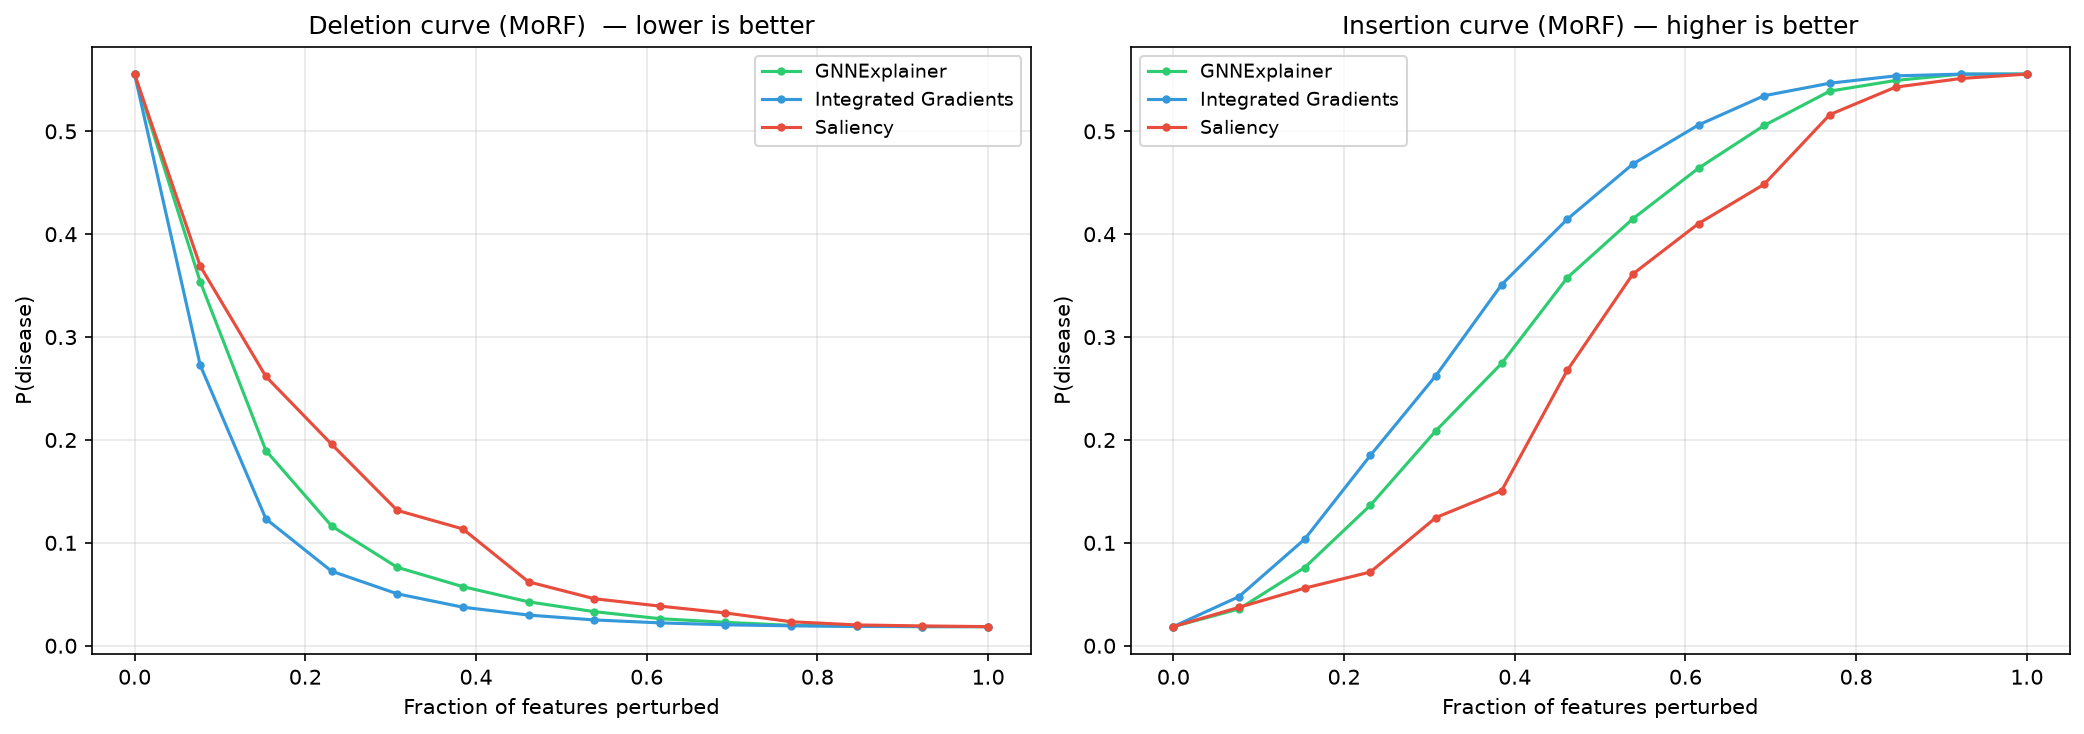
\includegraphics[width=\textwidth]{xai_deletion_insertion.png}
\caption{Deletion (left, lower is better) and insertion (right, higher is
better) curves under most-relevant-first perturbation. Integrated
Gradients produces the sharpest drop and fastest recovery.}
\label{fig:delins}
\end{figure*}




\subsection{Error analysis}
\label{sec:error}
Fig.~\ref{fig:error} shows that misclassifications concentrate near the
decision boundary: the model is rarely confidently wrong, which is
desirable in a screening context where borderline cases can be flagged for
clinician review. \begin{figure}[t]
\centering

\includegraphics[width=\columnwidth]{fig30_error_analysis.png}
\caption{Error analysis. Correct predictions are confident, whereas
misclassifications cluster around $P=0.5$, indicating calibrated
uncertainty rather than confident errors.}
\label{fig:error}
\end{figure}


\subsection{Cross-site transport within the UCI heart-disease collection}
\label{sec:external}
\textbf{Terminology and scope.} We refer to the Hungarian, Switzerland
and Long-Beach-VA cohorts as \emph{external} to the Cleveland cohort on
which every component is fit, and to this evaluation as external
validation, in the narrow sense that no observation from these three
cohorts is used at any stage of model development. We do not intend the
stronger sense in which the term is sometimes used---validation on a
cohort collected by an unrelated group, under an unrelated protocol, in
an unrelated era. All four cohorts are constituent databases of the same
UCI Heart Disease
collection~\cite{uci_heart,detrano1989}, assembled by coordinated
investigators using a shared variable
definition and recruitment protocol in the late 1980s. Site, and to some
degree the recruiting era, therefore differ across cohorts, but the
broader clinical and measurement lineage does not, and the transport
result below should be read as cross-site evaluation within one
historical data collection rather than validation against an independent
one.

\textbf{Feature availability constrains what can be validated.} The
primary 13-feature model cannot be transported: the non-Cleveland UCI
cohorts systematically do not record \texttt{ca} (95--99\% missing),
\texttt{thal} (42--90\%) or \texttt{slope} (14--65\%), and the Switzerland
\texttt{chol} column is entirely zero-encoded, a documented sentinel
rather than a measurement. Complete-case counts for the full feature
vector are 1/294 (Hungarian), 0/123 (Switzerland) and 1/200 (VA), so
cross-cohort transport evaluation of the full model is impossible in principle, not
merely inconvenient (Table~\ref{tab:extcohorts}). We therefore define a
\emph{transportable} subset of the eight variables recorded in all four
cohorts---\texttt{age}, \texttt{sex}, \texttt{cp}, \texttt{trestbps},
\texttt{restecg}, \texttt{thalach}, \texttt{exang} and
\texttt{oldpeak}---and retrain the identical architecture on Cleveland
restricted to those features. Discarding \texttt{chol} and \texttt{fbs}
costs little (target correlations $+0.085$ and $+0.025$), whereas
discarding \texttt{ca} ($+0.460$), \texttt{thal} ($+0.516$) and
\texttt{slope} ($+0.339$) is a genuine loss forced by data availability
rather than chosen. That cost is visible internally: cross-validated
ROC-AUC on Cleveland falls from $0.905\pm0.041$ (13 features) to
$0.840\pm0.038$ (8 features, Table~\ref{tab:extref}), which separates the
price of feature reduction from the price of cohort shift.

\textbf{Protocol.} The scaler, the correlation+MST graph, the network
weights and the decision threshold are all fit on Cleveland alone; each
external cohort is scored exactly once, baselines are transported under
the identical protocol, and the procedure is repeated over five seeds.
The transport, calibration and decision-curve analyses that follow
compare three models---the feature-node GCN, Logistic Regression and
Random Forest---rather than all seven of Table~\ref{tab:comparison}:
these are the strongest linear and ensemble baselines in distribution,
and holding the transported set to three keeps the five-seed $\times$
three-cohort protocol and its bootstrap intervals interpretable. The
boosted-tree baselines are reported in distribution only.

\textbf{Result.} The feature-node GCN attains a higher ROC-AUC than both
baselines on all three external cohorts (Hungarian $0.876\pm0.004$,
Switzerland $0.744\pm0.008$, VA $0.721\pm0.007$), so the sign of the
difference is positive in all six model--cohort comparisons
(Table~\ref{tab:external}, Fig.~\ref{fig:extauc}). On Hungarian the
transported AUC ($0.876$) exceeds the model's own internal Cleveland AUC
on the same eight features ($0.840$); we note this but do not read it as
superior transfer, since ROC-AUC is not comparable across cohorts of
different case mix. This contrasts with the in-distribution result of
Section~\ref{sec:results}, where the GCN was statistically
indistinguishable from the same baselines, and suggests that the graph
prior buys robustness to covariate and prevalence shift rather than
in-distribution accuracy: restricting message passing to statistically
related features appears to encode structure that is more stable across
populations than the marginal decision surfaces the tabular baselines
learn. Random Forest in particular degenerates toward majority-class
prediction under shift, its specificity falling to $0.39$, $0.20$ and
$0.11$ across the three cohorts, whereas the GCN retains a balanced
operating point; Logistic Regression retains comparable specificity but at
substantially lower AUC.

\textbf{The patient-similarity formulation transports less reliably.} We
transported the patient-similarity GNN of Section~\ref{sec:formulation}
under the identical protocol, with $k$ fixed at the value selected on
Cleveland and never re-tuned (Table~\ref{tab:patext}). The feature-node
model attains the higher ROC-AUC on two of three cohorts---Hungarian
($+0.011$) and VA ($+0.055$)---while Switzerland marginally favours the
patient-similarity model ($-0.009$, Table~\ref{tab:formext}); we report
that split result as it stands. The difference in \emph{failure mode} is
nonetheless stark: on VA the patient-similarity model degenerated to a
single-class predictor in all five seeds, labelling every patient diseased
(recall $1.000\pm0.000$, specificity $0.000\pm0.000$, MCC
$0.000\pm0.000$), and approached the same degeneracy on Switzerland
(specificity $0.150$), whereas the feature-node model retained a usable
operating point on both. Because the transductive model must rebuild its
neighbourhood graph from the external cohort itself, a shifted covariate
distribution reshapes the very structure over which messages pass; the
feature-node model instead re-uses a fixed, Cleveland-derived feature
topology unchanged.

\textbf{Statistical support, honestly stated.} DeLong's test on the
correlated ROC curves spans six comparisons (three cohorts $\times$ two
baselines), so we judge it on Holm-adjusted $p$-values
(Table~\ref{tab:extstats}). Only one survives correction: Logistic
Regression on Hungarian ($\Delta\mathrm{AUC}=+0.169$, raw
$p=5\times10^{-8}$, adjusted $p<10^{-4}$). The two comparisons nominally
significant before correction---VA against Logistic Regression ($+0.162$,
raw $p=0.022$) and Switzerland against Random Forest ($+0.126$, raw
$p=0.020$)---do not survive (both adjusted $p=0.100$). These $p$-values
must be read alongside the sampling uncertainty, which is severe on two
cohorts: Switzerland contributes only eight negative cases and VA thirty,
so a seed-to-seed standard deviation, which measures only initialisation
variability, drastically understates the true uncertainty. We therefore
computed a nested bootstrap ($B=2000$) resampling patients in a
class-stratified manner \emph{and} drawing over the five fitted models
(Table~\ref{tab:extboot}). The effect is large: the Switzerland AUC is
$0.745$ with a $95\%$ interval of $[0.543,0.927]$---a width of $0.38$
against a seed-only spread of $0.008$---so any conclusion from Switzerland
alone is weakly supported irrespective of the point estimate. Paired
bootstrap intervals for $\Delta$AUC (Table~\ref{tab:extbootdelta}) give
the most conservative summary: the advantage over Logistic Regression is
established on Hungarian ($+0.169$, $[+0.108,+0.231]$) and VA ($+0.151$,
$[+0.020,+0.289]$), while every remaining comparison, including all three
against Random Forest, has an interval containing zero. The Switzerland
contrast against Random Forest, which DeLong marks significant, has a
paired interval of $[-0.091,+0.215]$; with eight negative cases we regard
the bootstrap as more reliable and do not claim that advantage.

Per-cohort intervals are, however, the wrong instrument for the question
``does the advantage hold on transport as a whole?'', because each is
limited by its own negative count---eight for Switzerland, thirty for VA.
Combining them post hoc would require an independence assumption that is
false here: all three cohorts are scored by the \emph{same} fitted models,
so their errors are correlated through the shared fit. We therefore
re-ran the bootstrap jointly over all $548$ transported patients,
resampling stratified by cohort and class and drawing one model seed per
replicate for every cohort, so that the shared-fit correlation is carried
by the resampling scheme rather than assumed away
(Table~\ref{tab:extbootdelta}, pooled rows). Pooling raises precision
substantially---the interval against Logistic Regression narrows to
$[+0.075,+0.236]$---and the comparison against Random Forest becomes
$+0.050$, $[+0.004,+0.135]$. That lower bound is only $0.004$ above zero,
with bootstrap tail mass $P(\Delta\!\leq\!0)=0.015$; we verified that it
remains positive across five independent bootstrap seeds at $B=20{,}000$,
so it is not an artefact of a single draw, but we treat a margin of this
size as suggestive rather than decisive.

We therefore state the external finding as follows: the feature-node GCN
is \emph{directionally superior in all six model--cohort comparisons}, its
advantage over Logistic Regression is \emph{established on two of three
cohorts individually and on the pooled cohort}, and its advantage over
Random Forest is \emph{not established on any cohort individually and only
marginally on the pooled cohort}. We emphasise that pooling buys
precision, not independence: the pooled interval speaks to transport
across these three sites of one historical collection, and does not
substitute for validation on data collected under an unrelated protocol.

\textbf{Caveats.} Prevalence shifts from $46\%$ to $93\%$ across cohorts,
so threshold-dependent metrics are hard to interpret; Hungarian, with 292
complete cases and a $36\%$ prevalence closest to Cleveland's, is the most
trustworthy of the three and is also where the advantage is clearest.
Complete-case filtering is not neutral for VA: $60$ of $200$ records
($30.0\%$) are dropped and prevalence among retained cases ($78.6\%$) is
$4.1$ percentage points higher than in the full cohort ($74.5\%$),
indicating mild outcome-dependent missingness, whereas Hungarian and
Switzerland show no comparable shift ($<0.5$\,pp,
Table~\ref{tab:extcohorts}). No imputation is used at any stage, so this
selection effect, not an imputation artefact, is the source of any
residual bias on VA.

% ---- begin inlined: combined_patientext ----
\begin{table*}[t]
\centering
\caption{Transport of the patient-similarity formulation. Panel (a) reports its external performance; panel (b) contrasts it with the feature-node model per cohort.}
\label{tab:patext}
\label{tab:formext}
\footnotesize
\textbf{(a) Patient-similarity, transported}\\[2pt]
\resizebox{\textwidth}{!}{%
\begin{tabular}{lrrrrrrrrr}
\toprule
Cohort & Model & n & Accuracy & Precision & Recall & F1 & ROC-AUC & MCC & Specificity \\
\midrule
Hungarian & Patient-similarity GNN (k=15) & 292 & 0.7486 $\pm$ 0.0749 & 0.6312 $\pm$ 0.0911 & 0.8343 $\pm$ 0.0891 & 0.7093 $\pm$ 0.0493 & 0.8648 $\pm$ 0.0175 & 0.5277 $\pm$ 0.0893 & 0.7005 $\pm$ 0.1501 \\
Switzerland & Patient-similarity GNN (k=15) & 116 & 0.9103 $\pm$ 0.0372 & 0.9399 $\pm$ 0.0145 & 0.9667 $\pm$ 0.0579 & 0.9517 $\pm$ 0.0227 & 0.7537 $\pm$ 0.0693 & 0.0968 $\pm$ 0.1269 & 0.1500 $\pm$ 0.2424 \\
VA Long Beach & Patient-similarity GNN (k=15) & 140 & 0.7857 $\pm$ 0.0000 & 0.7857 $\pm$ 0.0000 & 1.0000 $\pm$ 0.0000 & 0.8800 $\pm$ 0.0000 & 0.6662 $\pm$ 0.0397 & 0.0000 $\pm$ 0.0000 & 0.0000 $\pm$ 0.0000 \\
\bottomrule
\end{tabular}
}
\vspace{7pt}
\textbf{(b) Contrast per cohort}\\[2pt]
\begin{tabular}{lrrr}
\toprule
Cohort & AUC feature-node & AUC patient-sim & $\Delta$AUC \\
\midrule
Hungarian & 0.8755 & 0.8648 & 0.0107 \\
Switzerland & 0.7444 & 0.7537 & -0.0093 \\
VA Long Beach & 0.7211 & 0.6662 & 0.0549 \\
\bottomrule
\end{tabular}
\end{table*}
%% ---- end inlined: combined_patientext ----
% ---- begin inlined: combined_extsetup ----
\begin{table*}[t]
\centering
\caption{External cohort setup. Panel (a) reports cohort availability under the 8-feature transportable set; panel (b) gives the internal Cleveland reference for that reduced model, separating the cost of feature reduction from the cost of cohort shift.}
\label{tab:extcohorts}
\label{tab:extref}
\footnotesize
\textbf{(a) Cohort availability}\\[2pt]
\resizebox{\textwidth}{!}{%
\begin{tabular}{lrrrrrrrrr}
\toprule
Cohort & Total records & Complete cases (8 features) & Missing (dropped) & Missing \% & Prevalence (all records) & Prevalence (complete cases) & Positive (n) & Negative (n) & Status \\
\midrule
Hungarian & 294 & 292 & 2 & 0.7 & 36.1\% & 36.0\% & 105 & 187 & evaluated \\
Switzerland & 123 & 116 & 7 & 5.7 & 93.5\% & 93.1\% & 108 & 8 & evaluated \\
VA Long Beach & 200 & 140 & 60 & 30.0 & 74.5\% & 78.6\% & 110 & 30 & evaluated \\
\bottomrule
\end{tabular}
}
\vspace{7pt}
\textbf{(b) Internal 8-feature reference}\\[2pt]
\resizebox{\textwidth}{!}{%
\begin{tabular}{lrrrrrr}
\toprule
Setting & Accuracy & Recall & F1 & ROC-AUC & MCC & Specificity \\
\midrule
Cleveland internal CV (8-feature) & 0.7275 $\pm$ 0.0783 & 0.8041 $\pm$ 0.0996 & 0.7333 $\pm$ 0.0463 & 0.8400 $\pm$ 0.0379 & 0.4819 $\pm$ 0.1210 & 0.6622 $\pm$ 0.2007 \\
\bottomrule
\end{tabular}
}
\end{table*}
%% ---- end inlined: combined_extsetup ----
% ---- begin inlined: combined_extresult ----
\begin{table*}[t]
\centering
\caption{External validation results. Panel (a) reports transported performance per cohort (mean $\pm$ std over 5 seeds); panel (b) reports the corresponding DeLong and McNemar comparisons with Holm correction.}
\label{tab:external}
\label{tab:extstats}
\footnotesize
\textbf{(a) Transported performance}\\[2pt]
\resizebox{\textwidth}{!}{%
\begin{tabular}{lrrrrrrr}
\toprule
Cohort & Model & n & Recall & F1 & ROC-AUC & MCC & Specificity \\
\midrule
Hungarian & GCN (Ours) & 292 & 0.6629 $\pm$ 0.0712 & 0.7080 $\pm$ 0.0195 & 0.8755 $\pm$ 0.0037 & 0.5715 $\pm$ 0.0075 & 0.8845 $\pm$ 0.0456 \\
Hungarian & Logistic Regression & 292 & 0.3810 $\pm$ 0.1927 & 0.4361 $\pm$ 0.1069 & 0.7060 $\pm$ 0.0025 & 0.2817 $\pm$ 0.0324 & 0.8492 $\pm$ 0.1262 \\
Hungarian & Random Forest & 292 & 0.9219 $\pm$ 0.0904 & 0.6201 $\pm$ 0.0461 & 0.8413 $\pm$ 0.0059 & 0.3536 $\pm$ 0.0940 & 0.3904 $\pm$ 0.2096 \\
Switzerland & GCN (Ours) & 116 & 0.5907 $\pm$ 0.0773 & 0.7286 $\pm$ 0.0628 & 0.7444 $\pm$ 0.0083 & 0.1384 $\pm$ 0.0482 & 0.6750 $\pm$ 0.0612 \\
Switzerland & Logistic Regression & 116 & 0.4556 $\pm$ 0.1819 & 0.5944 $\pm$ 0.1720 & 0.6287 $\pm$ 0.0195 & 0.0828 $\pm$ 0.0273 & 0.7000 $\pm$ 0.1696 \\
Switzerland & Random Forest & 116 & 0.8852 $\pm$ 0.1374 & 0.9042 $\pm$ 0.0751 & 0.6748 $\pm$ 0.0724 & 0.0315 $\pm$ 0.1200 & 0.2000 $\pm$ 0.3410 \\
VA Long Beach & GCN (Ours) & 140 & 0.7545 $\pm$ 0.0551 & 0.7994 $\pm$ 0.0229 & 0.7211 $\pm$ 0.0068 & 0.2451 $\pm$ 0.0700 & 0.5200 $\pm$ 0.1343 \\
VA Long Beach & Logistic Regression & 140 & 0.5309 $\pm$ 0.2310 & 0.6091 $\pm$ 0.1767 & 0.5697 $\pm$ 0.0055 & 0.0545 $\pm$ 0.0120 & 0.5267 $\pm$ 0.2332 \\
VA Long Beach & Random Forest & 140 & 0.9436 $\pm$ 0.1082 & 0.8606 $\pm$ 0.0420 & 0.6676 $\pm$ 0.0198 & 0.1160 $\pm$ 0.0661 & 0.1133 $\pm$ 0.1771 \\
\bottomrule
\end{tabular}
}
\vspace{7pt}
\textbf{(b) Statistical comparison}\\[2pt]
\resizebox{\textwidth}{!}{%
\begin{tabular}{lrrrrrrrrrr}
\toprule
Cohort & Comparison & AUC$_{\mathrm{GCN}}$ & AUC$_{\mathrm{other}}$ & $\Delta$AUC & DeLong $p$ & McNemar $p$ & Holm p (DeLong) & Sig. Holm (DeLong) & Holm p (McNemar) & Sig. Holm (McNemar) \\
\midrule
Hungarian & GCN vs Logistic Regression & 0.8737 & 0.7046 & 0.1691 & 5.1e-08 & 1.4e-05 & 0.0 & yes & 0.0001 & yes \\
Hungarian & GCN vs Random Forest & 0.8737 & 0.8402 & 0.0335 & 0.1459 & 4.72e-10 & 0.3801 & no & 0.0 & yes \\
Switzerland & GCN vs Logistic Regression & 0.7407 & 0.5914 & 0.1493 & 0.3626 & 1.96e-05 & 0.3801 & no & 0.0001 & yes \\
Switzerland & GCN vs Random Forest & 0.7407 & 0.6152 & 0.1256 & 0.02 & 1.3e-09 & 0.1 & no & 0.0 & yes \\
VA Long Beach & GCN vs Logistic Regression & 0.7255 & 0.5636 & 0.1618 & 0.0219 & 0.2807 & 0.1 & no & 0.2807 & no \\
VA Long Beach & GCN vs Random Forest & 0.7255 & 0.6385 & 0.087 & 0.1267 & 0.0489 & 0.3801 & no & 0.0978 & no \\
\bottomrule
\end{tabular}
}
\end{table*}
%% ---- end inlined: combined_extresult ----
% ---- begin inlined: combined_bootstrap ----
\begin{table*}[t]
\centering
\caption{Paired patient-level bootstrap on the external cohorts. Panel (a) reports per-model ROC-AUC with percentile intervals; panel (b) reports the paired differences against the feature-node model. The pooled rows of panel (b) resample the three cohorts jointly, stratified by cohort and class, so that model-selection and sampling uncertainty are propagated across all $548$ transported patients in a single interval rather than combined post hoc; the pooled AUC is the complete-case-weighted mean of the within-cohort AUCs, which avoids crediting a model for between-cohort prevalence differences. \textsuperscript{$\dagger$}This interval excludes zero but only marginally (lower bound $+0.004$, bootstrap tail mass $P(\Delta\!\leq\!0)=0.015$); it is stable across five independent bootstrap seeds at $B=20{,}000$, and we read it as suggestive rather than decisive.}
\label{tab:extboot}
\label{tab:extbootdelta}
\footnotesize
\textbf{(a) Bootstrap ROC-AUC}\\[2pt]
\begin{tabular}{lrrrrr}
\toprule
Cohort & Model & n (pos/neg) & AUC & 95\% CI & CI width \\
\midrule
Hungarian & GCN (Ours) & 105/187 & 0.875 & [0.829, 0.918] & 0.088 \\
Hungarian & Logistic Regression & 105/187 & 0.706 & [0.642, 0.767] & 0.125 \\
Hungarian & Random Forest & 105/187 & 0.841 & [0.786, 0.891] & 0.105 \\
Switzerland & GCN (Ours) & 108/8 & 0.745 & [0.543, 0.927] & 0.384 \\
Switzerland & Logistic Regression & 108/8 & 0.628 & [0.392, 0.833] & 0.441 \\
Switzerland & Random Forest & 108/8 & 0.678 & [0.430, 0.897] & 0.467 \\
VA Long Beach & GCN (Ours) & 110/30 & 0.722 & [0.622, 0.813] & 0.191 \\
VA Long Beach & Logistic Regression & 110/30 & 0.571 & [0.455, 0.688] & 0.233 \\
VA Long Beach & Random Forest & 110/30 & 0.669 & [0.553, 0.772] & 0.219 \\
\bottomrule
\end{tabular}
\vspace{7pt}
\textbf{(b) Paired differences}\\[2pt]
\begin{tabular}{lrrrr}
\toprule
Cohort & Comparison & $\Delta$AUC & 95\% CI & Excludes zero \\
\midrule
Hungarian & GCN $-$ Logistic Regression & 0.169 & [+0.108, +0.231] & yes \\
Hungarian & GCN $-$ Random Forest & 0.034 & [-0.007, +0.075] & no \\
Switzerland & GCN $-$ Logistic Regression & 0.116 & [-0.184, +0.407] & no \\
Switzerland & GCN $-$ Random Forest & 0.067 & [-0.091, +0.215] & no \\
VA Long Beach & GCN $-$ Logistic Regression & 0.151 & [+0.020, +0.289] & yes \\
VA Long Beach & GCN $-$ Random Forest & 0.052 & [-0.032, +0.156] & no \\
\midrule
% From the JOINT pooled bootstrap: run_external_bootstrap.py --pooled
% (stratified estimand; B=2000). Robustness at B=20000 across five RNG
% seeds in check_pooled_robustness.py: the Random Forest lower bound stays
% in [+0.003, +0.004] on every seed, so "yes" is stable rather than an
% artefact of one draw -- but it is marginal and the text says so.
Pooled external cohorts & GCN $-$ Logistic Regression & 0.153 & [+0.075, +0.236] & yes \\
Pooled external cohorts & GCN $-$ Random Forest & 0.050 & [+0.004, +0.135] & yes\textsuperscript{$\dagger$} \\
\bottomrule
\end{tabular}
\end{table*}
%% ---- end inlined: combined_bootstrap ----

\begin{figure*}[t]
\centering

\includegraphics[width=\textwidth]{fig31_external_auc.png}
\caption{Cross-cohort transport evaluation. Left: ROC-AUC by cohort for the transported
models (mean$\pm$std over five seeds); the feature-node GCN leads on all
three cohorts. Right: specificity under distribution shift; Random Forest
degenerates toward majority-class prediction while the GCN retains a
balanced operating point.}
\label{fig:extauc}
\end{figure*}

\subsection{\texorpdfstring{$\tau$}{Tau}-regime analysis of graph
connectivity}
\label{sec:tauregime}
The internal ablation found no benefit from the graph, and at our
operating point the MST is inert; both could be read as evidence that the
topology is decorative. We tested an alternative reading---that its
contribution is transportability rather than in-distribution accuracy, and
is therefore invisible to any internal experiment. Whether the MST acts at
all depends jointly on the threshold and the feature set: the 13-feature
graph stays connected for $\tau\le0.15$ and fragments from $\tau=0.20$,
whereas the reduced 8-feature transportable set already fragments at
$\tau=0.15$. This retrospectively explains the null ``w/o MST'' ablation
row, because at $\tau=0.15$ on 13 features the two conditions describe the
identical graph. Repeating the transport protocol of
Section~\ref{sec:external} at $\tau=0.20$, where the MST is active, the
internal and external orderings dissociate: internally the ranking is flat
and slightly favours the edgeless model (validation ROC-AUC $0.8293$
against $0.8276$), whereas externally Corr+MST attains the highest ROC-AUC
on all three cohorts and the edgeless model falls to $0.6343$ on
Switzerland against $0.7433$. Page's trend test for the ordered
alternative is significant pooled ($L=406$, $p=1.4\times10^{-9}$ over $30$
seed$\times$cohort blocks)~\cite{page1963}, and a fully connected graph,
which is also a single component and therefore isolates selectivity from
connectivity, is significantly worse than Corr+MST on all three cohorts
($\Delta$AUC $+0.0117$ to $+0.0572$, all $p\le0.006$). What transports is
thus a \emph{sparse, correlation-selective} topology that is also
connected---not density, and not connectivity on its own. We bound the
claim to what the evidence supports: these tests are computed over random
initialisations, and under paired patient-level bootstrap only $3$ of $9$
contrasts exclude zero, none surviving Holm correction of the DeLong
tests, with modest effect sizes ($\Delta$AUC $+0.005$ to $+0.057$). We
therefore describe this only as \emph{suggestive evidence} that a
sparse, connected topology may be more favourable under distribution
shift, consistent in direction across three cohorts and reproducibly
across initialisations, with patient-level confidence established on the
best-powered cohort alone. We do not claim that the MST improves prediction; internally it
does not, and we retain it at $\tau=0.15$ as a connectivity safeguard, as
stated in Section~\ref{sec:mst}. The complete tables for this analysis
accompany the released code.

\section{Discussion}
We organise the discussion around the three properties set out in
Section~\ref{sec:intro}, then state what the evidence does not support.

\textbf{P1: Representation.} The feature-node graph turns an implicit
modelling assumption into an explicit, inspectable object: the topology is
available for spectral and centrality analysis \emph{before} any training
occurs (Section~\ref{sec:graph}), so the structure a clinician is asked to
trust can be examined independently of model fit---a property no tabular
baseline offers. Downstream, three mechanistically distinct attribution
methods converge on similar rankings (GNNExplainer and Integrated
Gradients: Spearman $\rho=0.80$, top-$k$ Jaccard $0.59$) that align with
established cardiovascular risk factors. Convergence across methods
matters more than any single attribution: it indicates the explanation
reflects the learned function rather than an artefact of one explainer.
The errors that remain concentrate near the decision boundary
(Section~\ref{sec:error}), which is the desirable failure profile for a
decision aid that defers uncertain cases rather than one that fails
confidently.

\textbf{P2: Deployability.} Because each patient is an independent graph,
inference is inductive by construction: the topology learned on the
development cohort is applied unchanged, and a single patient can be
scored with no cohort present. This is not a theoretical nicety. The
conventional patient-similarity GNN we implement as a baseline must first
construct a $k$-nearest-neighbour graph over whatever cohort it is asked
to score (Section~\ref{sec:formulation}); it therefore cannot score an
isolated referral at all, and its predictions for a given patient depend
on which other patients happen to be present. The feature-node model
carries none of that coupling: scoring patients individually reproduces
batch predictions to $3\times10^{-8}$ at $2.6$\,ms each, from an
$11.4$\,KB model (Section~\ref{sec:deploy}). It is also the best-calibrated
model out-of-fold and the one whose calibration best survives transport at
realistic prevalence---a property that matters more than discrimination
for a tool intended to report risk rather than rank patients. Where it
does \emph{not} yet earn its place is clinical utility on high-prevalence
cohorts: on Switzerland and VA no model improves on treating every
patient, so our demonstrated utility rests on Hungarian alone.

\textbf{P3: Transportability.} Fitting every component on Cleveland and
touching each external cohort once, the feature-node model attains the
higher ROC-AUC in all six model--cohort comparisons, though paired
bootstrap intervals establish this only against Logistic Regression and
only on two cohorts (Section~\ref{sec:external}). The more robust signal
is the difference in \emph{failure mode}: Random Forest drifts toward
majority-class prediction under shift, its specificity falling to $0.39$,
$0.20$ and $0.11$, and the patient-similarity GNN collapses entirely on
VA, labelling every patient diseased, whereas the feature-node model
retains a usable operating point throughout. We offer a mechanism: a model
that must rebuild its graph from the target cohort inherits that cohort's
distributional distortion into the very structure over which messages
pass, whereas a fixed feature topology derived from the development cohort
does not. That mechanism makes a testable prediction---degrading the
topology should hurt transport while leaving in-distribution accuracy
untouched---and Section~\ref{sec:tauregime} provides suggestive evidence
consistent with it: a fully connected graph transports worse despite
being equally connected, implicating \emph{selective} sparsity rather
than connectivity alone. The effect is modest and, at the patient level,
established only on the best-powered cohort, with no pairwise contrast
surviving Holm correction of the DeLong tests; it is nonetheless the most
direct evidence we have that the graph is doing work, and evidence no
in-distribution experiment in this paper could have produced.

\textbf{What the evidence does not support.} Two claims we might have
made, and do not. First, accuracy: the model is statistically
indistinguishable from all six classical baselines in-distribution,
including the two modern gradient-boosted-tree models (XGBoost,
LightGBM), and we report that parity as a finding rather than minimising
it. Second, architecture: substituting GAT, GraphSAGE or GIN
changes no metric significantly, so the contribution cannot be attributed
to the convolution. What remains, and what the ablation localises, is the
graph \emph{construction}---selective, correlation-derived sparsity, which
outperforms both random and fully connected topologies of comparable size.
More broadly, our results caution that on small, near-balanced clinical
cohorts differences between well-tuned models are usually within noise.
This matters for interpreting the many prior studies on this same
cohort that report high headline accuracies from hybrid or ensemble
pipelines without paired significance testing across a shared
protocol~\cite{mohan2019hybrid,latha2019ensemble}: without such testing
it cannot be established whether the reported margins exceed
split-to-split variation. Only a strictly shared protocol with
significance testing distinguishes genuine improvement from favourable
splitting, and reporting a model's non-superiority is often the more
informative result.
Table~\ref{tab:literature} positions our formulation against
representative paradigms.

% ---- begin inlined: table_literature_comparison ----
\begin{table*}[t]
\centering
\caption{Qualitative comparison with representative paradigms.}
\label{tab:literature}
\footnotesize
\begin{tabular}{p{2.6cm}p{2.0cm}p{3.0cm}p{1.6cm}p{3.0cm}}
\toprule
Paradigm & Reported accuracy regime & Explainability & Inference mode & Interpretability notes \\
\midrule
Classical tabular ML~\cite{mohan2019hybrid,latha2019ensemble} & High & None (post-hoc only) & N/A & Transparent at coefficient/importance level \\
Patient-similarity GNN~\cite{parisot2018disease} & Moderate--High & Node/edge masks on the population graph & Transductive & Explains via cohort neighbours, not features \\
Feature-node GCN (Ours) & Comparable to classical ML & GNNExplainer + Integrated Gradients + Saliency (8 metrics) & Inductive & Exposes feature-level interaction structure \\
\bottomrule
\end{tabular}
\end{table*}
%% ---- end inlined: table_literature_comparison ----

\section{Limitations}
\emph{(i)} The Cleveland cohort is small ($n=303$) and single-centre, and
the near-ceiling AUC leaves little separation between models, so accuracy
parity with strong baselines is expected. \emph{(ii)} Each node carries a
single scalar feature, which provably limits the expressive advantage of
message passing: the layer-1 node representation is rank-one in direction
by construction and reaches an effective rank of only $1.73$ out of $13$
after two layers (Section~\ref{sec:mechanism}). Consistent with this, the
graph does not significantly outperform independent feature processing, so
its principal value is representational and explanatory rather than
predictive. The obvious remedy---richer node features---is not
straightforward: a learnable per-feature identity embedding raises the
effective rank only when the graph is removed, and with edges present
message passing smooths the added identity away and degrades accuracy
monotonically with edge density. Lifting this ceiling therefore requires
an aggregation scheme that preserves node identity, not merely a wider
node encoding, and we identify that as the open problem rather than a
routine extension. \emph{(iii)} Pearson correlation captures only linear
feature dependence and may miss nonlinear interactions;
mutual-information or copula-based graphs are promising alternatives.
\emph{(iv)} The MST guarantees connectivity but does not improve internal
accuracy: at the operating threshold it adds no edges at all. Under
distribution shift an MST-supported sparse topology is associated with
better transport (Section~\ref{sec:tauregime}), but that evidence is
limited---the effect is modest, established at the patient level only on
the best-powered cohort, and no pairwise contrast survives correction for
multiple comparisons---so we treat transportability as directionally
supported rather than established. The construction rule is likewise not
empirically decisive on this cohort: a global correlation cut-off and a
per-node $k$-NN rule of comparable density are indistinguishable after
correction (Section~\ref{sec:construction}), so our preference rests on
parsimony and interpretability rather than measured performance.
\emph{(v)} The feature graph is small (thirteen nodes), bounding the depth
of useful message passing. \emph{(vi)} No temporal or longitudinal
information is modelled. \emph{(vii)} Cross-site validation is necessarily
restricted to an eight-feature model, because \texttt{ca}, \texttt{thal}
and \texttt{slope} are not recorded in the other cohorts; the full
13-feature model reported in Section~\ref{sec:results} therefore remains
validated only internally. Moreover, the Hungarian, Switzerland and VA
cohorts are not independent external data in the strongest sense: they
are constituent databases of the same UCI Heart Disease
collection~\cite{uci_heart,detrano1989} as Cleveland, sharing variable
definitions and recruitment era, so this evaluation demonstrates
cross-site robustness rather than validation against an unrelated
population (Section~\ref{sec:external}). \emph{(viii)} Two of the three external cohorts
are severely imbalanced (eight and thirty negative cases), so their
estimates carry very wide uncertainty---the bootstrap $95\%$ interval for
the Switzerland AUC spans $[0.543,0.927]$---and no comparison against
Random Forest excludes zero; where DeLong's test and the bootstrap
disagree we defer to the bootstrap, since asymptotic tests are unreliable
with eight negative cases. \emph{(ix)} The advantage over the
patient-similarity formulation is partial rather than uniform:
in-distribution it reaches significance in only one of three seeds, and on
transport that model attains a marginally higher AUC on Switzerland, so
our claim rests on the difference in failure mode and on the
inductive/transductive distinction, not on a uniform margin. \emph{(x)} We
compared four message-passing operators but did not tune each one's
hyperparameters separately. \emph{(xi)} Decision-curve analysis
establishes net benefit over the treat-all strategy on Hungarian only; on
Switzerland ($93\%$ prevalence) and VA ($79\%$) no model, ours included,
improves on treating every patient, so our clinical-utility evidence rests
on a single external cohort. \emph{(xii)} Calibration was assessed but not
corrected; recalibration would likely improve the poorly calibrated
external estimates.

\section{Conclusion}
When candidate models on a small clinical cohort are statistically tied on
accuracy---as they are here---the decision between them should turn on
representation, deployability and transportability, and we evaluated a
feature-node graph formulation against exactly those criteria. The
formulation converts a modelling assumption into an inspectable topology
that is validated spectrally before training and explained by three
concordant attribution methods; it is inductive by construction, scoring
an isolated patient from an $11.4$\,KB, $1{,}281$-parameter model where
the patient-similarity baseline cannot score such a patient at all; and it
attains the higher ROC-AUC in all six external comparisons while retaining
a usable operating point where the baselines drift toward majority-class
prediction. We bound both claims honestly: the transport advantage is
established only against Logistic Regression and only on two cohorts, and
on accuracy we report a null result and decline to dress it otherwise.
Substituting GAT, GraphSAGE or GIN changes no metric significantly, which
localises whatever contribution exists to the graph construction rather
than the operator. We hope the honest positioning and full reproducibility
of this study serve as a useful template for evaluating graph-based models
on small clinical datasets, where the temptation to report a fractional
accuracy gain is strong and the evidence for it is usually absent. Future
work will pursue richer node features, nonlinear dependence graphs,
calibrated risk estimates, and prospective multi-centre validation on
cohorts that record the full feature set.

%% ---- begin inlined bibliography (IEEEtran.bst output, self-contained) ----
% Generated by IEEEtran.bst, version: 1.14 (2015/08/26)
\begin{thebibliography}{10}
\providecommand{\url}[1]{#1}
\csname url@samestyle\endcsname
\providecommand{\newblock}{\relax}
\providecommand{\bibinfo}[2]{#2}
\providecommand{\BIBentrySTDinterwordspacing}{\spaceskip=0pt\relax}
\providecommand{\BIBentryALTinterwordstretchfactor}{4}
\providecommand{\BIBentryALTinterwordspacing}{\spaceskip=\fontdimen2\font plus
\BIBentryALTinterwordstretchfactor\fontdimen3\font minus
  \fontdimen4\font\relax}
\providecommand{\BIBforeignlanguage}[2]{{%
\expandafter\ifx\csname l@#1\endcsname\relax
\typeout{** WARNING: IEEEtran.bst: No hyphenation pattern has been}%
\typeout{** loaded for the language `#1'. Using the pattern for}%
\typeout{** the default language instead.}%
\else
\language=\csname l@#1\endcsname
\fi
#2}}
\providecommand{\BIBdecl}{\relax}
\BIBdecl

\bibitem{world2021cvd}
{World Health Organization}, ``Cardiovascular diseases (cvds) fact sheet,''
  World Health Organization, Geneva, Switzerland, Tech. Rep., 2021.

\bibitem{petch2022opening}
J.~Petch, S.~Di, and W.~Nelson, ``Opening the black box: The promise and
  limitations of explainable machine learning in cardiology,'' \emph{Canadian
  Journal of Cardiology}, vol.~38, no.~2, pp. 204--213, 2022.

\bibitem{ahmad2018survey}
M.~A. Ahmad, C.~Eckert, and A.~Teredesai, ``Interpretable machine learning in
  healthcare,'' \emph{IEEE Intelligent Informatics Bulletin}, 2018.

\bibitem{kipf2017gcn}
T.~N. Kipf and M.~Welling, ``Semi-supervised classification with graph
  convolutional networks,'' in \emph{International Conference on Learning
  Representations (ICLR)}, 2017.

\bibitem{zhou2020gnnreview}
J.~Zhou, G.~Cui, S.~Hu, Z.~Zhang, C.~Yang, Z.~Liu, L.~Wang, C.~Li, and M.~Sun,
  ``Graph neural networks: A review of methods and applications,'' \emph{AI
  Open}, vol.~1, pp. 57--81, 2020.

\bibitem{velickovic2018gat}
P.~Veli{\v{c}}kovi{\'c}, G.~Cucurull, A.~Casanova, A.~Romero, P.~Li{\`o}, and
  Y.~Bengio, ``Graph attention networks,'' in \emph{International Conference on
  Learning Representations (ICLR)}, 2018.

\bibitem{hamilton2017graphsage}
W.~L. Hamilton, R.~Ying, and J.~Leskovec, ``Inductive representation learning
  on large graphs,'' in \emph{Advances in Neural Information Processing Systems
  (NeurIPS)}, 2017.

\bibitem{xu2019gin}
K.~Xu, W.~Hu, J.~Leskovec, and S.~Jegelka, ``How powerful are graph neural
  networks?'' in \emph{International Conference on Learning Representations
  (ICLR)}, 2019.

\bibitem{parisot2018disease}
S.~Parisot, S.~I. Ktena, E.~Ferrante, M.~Lee, R.~Guerrero, B.~Glocker, and
  D.~Rueckert, ``Disease prediction using graph convolutional networks:
  Application to autism spectrum disorder and alzheimer's disease,''
  \emph{Medical Image Analysis}, vol.~48, pp. 117--130, 2018.

\bibitem{li2022graphrepbiomed}
M.~M. Li, K.~Huang, and M.~Zitnik, ``Graph representation learning in
  biomedicine and healthcare,'' \emph{Nature Biomedical Engineering}, vol.~6,
  no.~12, pp. 1353--1369, 2022.

\bibitem{ektefaie2023multimodalgraphs}
Y.~Ektefaie, G.~Dasoulas, A.~Noori, M.~Farhat, and M.~Zitnik, ``Multimodal
  learning with graphs,'' \emph{Nature Machine Intelligence}, vol.~5, no.~4,
  pp. 340--350, 2023.

\bibitem{yan2023t2gformer}
J.~Yan, J.~Chen, Y.~Wu, D.~Z. Chen, and J.~Wu, ``{T2G-FORMER}: Organizing
  tabular features into relation graphs promotes heterogeneous feature
  interaction,'' in \emph{Proceedings of the AAAI Conference on Artificial
  Intelligence}, vol.~37, no.~9, 2023, pp. 10\,720--10\,728.

\bibitem{villaizan2024gnncontextual}
M.~Villaiz{\'a}n-Vallelado, M.~Salvatori, B.~Carro, and A.~J.
  Sanchez-Esguevillas, ``Graph neural network contextual embedding for deep
  learning on tabular data,'' \emph{Neural Networks}, vol. 173, p. 106180,
  2024.

\bibitem{li2025gnntabularsurvey}
C.-T. Li, Y.-C. Tsai, C.-Y. Chen, and J.~C. Liao, ``Graph neural networks for
  tabular data learning: A survey with taxonomy and directions,'' \emph{ACM
  Computing Surveys}, vol.~58, no.~1, pp. 1--51, 2025.

\bibitem{badaro2023transformerstabular}
G.~Badaro, M.~Saeed, and P.~Papotti, ``Transformers for tabular data
  representation: A survey of models and applications,'' \emph{Transactions of
  the Association for Computational Linguistics}, vol.~11, pp. 227--249, 2023.

\bibitem{hollmann2025tabpfn}
N.~Hollmann, S.~M{\"u}ller, L.~Purucker, A.~Krishnakumar, M.~K{\"o}rfer, S.~B.
  Hoo, R.~T. Schirrmeister, and F.~Hutter, ``Accurate predictions on small data
  with a tabular foundation model,'' \emph{Nature}, vol. 637, no. 8045, pp.
  319--326, 2025.

\bibitem{samek2021xai}
W.~Samek, G.~Montavon, S.~Lapuschkin, C.~J. Anders, and K.-R. M{\"u}ller,
  ``Explaining deep neural networks and beyond: A review of methods and
  applications,'' \emph{Proceedings of the IEEE}, vol. 109, no.~3, pp.
  247--278, 2021.

\bibitem{lisboa2023interpretablecoming}
P.~Lisb{\^o}a, S.~Saralajew, A.~Vellido, R.~Fern{\'a}ndez-Domenech, and
  T.~Villmann, ``The coming of age of interpretable and explainable machine
  learning models,'' \emph{Neurocomputing}, vol. 535, pp. 25--39, 2023.

\bibitem{poncebobadilla2024shap}
A.~V. Ponce~Bobadilla, V.~Schmitt, C.~S. Maier, S.~Mensing, and S.~Stodtmann,
  ``Practical guide to {SHAP} analysis: Explaining supervised machine learning
  model predictions in drug development,'' \emph{Clinical and Translational
  Science}, vol.~17, no.~11, p. e70056, 2024.

\bibitem{ying2019gnnexplainer}
R.~Ying, D.~Bourgeois, J.~You, M.~Zitnik, and J.~Leskovec, ``{GNNExplainer}:
  Generating explanations for graph neural networks,'' in \emph{Advances in
  Neural Information Processing Systems (NeurIPS)}, 2019.

\bibitem{sundararajan2017ig}
M.~Sundararajan, A.~Taly, and Q.~Yan, ``Axiomatic attribution for deep
  networks,'' in \emph{International Conference on Machine Learning (ICML)},
  2017.

\bibitem{simonyan2014saliency}
K.~Simonyan, A.~Vedaldi, and A.~Zisserman, ``Deep inside convolutional
  networks: Visualising image classification models and saliency maps,'' in
  \emph{ICLR Workshop}, 2014.

\bibitem{yeh2019infidelity}
C.-K. Yeh, C.-Y. Hsieh, A.~S. Suggala, D.~I. Inouye, and P.~Ravikumar, ``On the
  (in)fidelity and sensitivity of explanations,'' \emph{Advances in Neural
  Information Processing Systems (NeurIPS)}, 2019.

\bibitem{uci_heart}
A.~Janosi, W.~Steinbrunn, M.~Pfisterer, and R.~Detrano, ``{Heart Disease},''
  UCI Machine Learning Repository, 1988, dOI: 10.24432/C52P4X.

\bibitem{detrano1989}
R.~Detrano, A.~J{\'a}nosi, W.~Steinbrunn, M.~Pfisterer, J.-J. Schmid,
  S.~Sandhu, K.~H. Guppy, S.~Lee, and V.~Froelicher, ``International
  application of a new probability algorithm for the diagnosis of coronary
  artery disease,'' \emph{The American Journal of Cardiology}, vol.~64, no.~5,
  pp. 304--310, 1989.

\bibitem{prim1957}
R.~C. Prim, ``Shortest connection networks and some generalizations,''
  \emph{The Bell System Technical Journal}, vol.~36, no.~6, pp. 1389--1401,
  1957.

\bibitem{fiedler1973}
M.~Fiedler, ``Algebraic connectivity of graphs,'' \emph{Czechoslovak
  Mathematical Journal}, vol.~23, no.~2, pp. 298--305, 1973.

\bibitem{chen2016xgboost}
T.~Chen and C.~Guestrin, ``{XGBoost}: A scalable tree boosting system,'' in
  \emph{Proceedings of the 22nd ACM SIGKDD International Conference on
  Knowledge Discovery and Data Mining (KDD)}, 2016, pp. 785--794.

\bibitem{ke2017lightgbm}
G.~Ke, Q.~Meng, T.~Finley, T.~Wang, W.~Chen, W.~Ma, Q.~Ye, and T.-Y. Liu,
  ``{LightGBM}: A highly efficient gradient boosting decision tree,'' in
  \emph{Advances in Neural Information Processing Systems (NeurIPS)}, vol.~30,
  2017, pp. 3146--3154.

\bibitem{matthews1975}
B.~W. Matthews, ``Comparison of the predicted and observed secondary structure
  of {T4} phage lysozyme,'' \emph{Biochimica et Biophysica Acta (BBA) - Protein
  Structure}, vol. 405, no.~2, pp. 442--451, 1975.

\bibitem{mcnemar1947}
Q.~McNemar, ``Note on the sampling error of the difference between correlated
  proportions or percentages,'' \emph{Psychometrika}, vol.~12, no.~2, pp.
  153--157, 1947.

\bibitem{wilcoxon1945}
F.~Wilcoxon, ``Individual comparisons by ranking methods,'' \emph{Biometrics
  Bulletin}, vol.~1, no.~6, pp. 80--83, 1945.

\bibitem{holm1979}
S.~Holm, ``A simple sequentially rejective multiple test procedure,''
  \emph{Scandinavian Journal of Statistics}, vol.~6, no.~2, pp. 65--70, 1979.

\bibitem{paszke2019pytorch}
A.~Paszke \emph{et~al.}, ``{PyTorch}: An imperative style, high-performance
  deep learning library,'' in \emph{Advances in Neural Information Processing
  Systems (NeurIPS)}, 2019.

\bibitem{fey2019pyg}
M.~Fey and J.~E. Lenssen, ``Fast graph representation learning with {PyTorch
  Geometric},'' in \emph{ICLR Workshop on Representation Learning on Graphs and
  Manifolds}, 2019.

\bibitem{pedregosa2011scikit}
F.~Pedregosa \emph{et~al.}, ``Scikit-learn: Machine learning in {Python},''
  \emph{Journal of Machine Learning Research}, vol.~12, pp. 2825--2830, 2011.

\bibitem{delong1988}
E.~R. DeLong, D.~M. DeLong, and D.~L. Clarke-Pearson, ``Comparing the areas
  under two or more correlated receiver operating characteristic curves: A
  nonparametric approach,'' \emph{Biometrics}, vol.~44, no.~3, pp. 837--845,
  1988.

\bibitem{brier1950}
G.~W. Brier, ``Verification of forecasts expressed in terms of probability,''
  \emph{Monthly Weather Review}, vol.~78, no.~1, pp. 1--3, 1950.

\bibitem{naeini2015ece}
M.~P. Naeini, G.~F. Cooper, and M.~Hauskrecht, ``Obtaining well calibrated
  probabilities using {Bayesian} binning,'' in \emph{Proceedings of the AAAI
  Conference on Artificial Intelligence}, vol.~29, no.~1, 2015, pp. 2901--2907.

\bibitem{vickers2006dca}
A.~J. Vickers and E.~B. Elkin, ``Decision curve analysis: A novel method for
  evaluating prediction models,'' \emph{Medical Decision Making}, vol.~26,
  no.~6, pp. 565--574, 2006.

\bibitem{page1963}
E.~B. Page, ``Ordered hypotheses for multiple treatments: A significance test
  for linear ranks,'' \emph{Journal of the American Statistical Association},
  vol.~58, no. 301, pp. 216--230, 1963.

\bibitem{mohan2019hybrid}
S.~Mohan, C.~Thirumalai, and G.~Srivastava, ``Effective heart disease
  prediction using hybrid machine learning techniques,'' \emph{IEEE Access},
  vol.~7, pp. 81\,542--81\,554, 2019.

\bibitem{latha2019ensemble}
C.~B.~C. Latha and S.~C. Jeeva, ``Improving the accuracy of prediction of heart
  disease risk based on ensemble classification techniques,'' \emph{Informatics
  in Medicine Unlocked}, vol.~16, p. 100203, 2019.

\end{thebibliography}
%%%% ---- end inlined bibliography ----

%% ------------------------- SUBMISSION-TODO -------------------------
%% IEEE Access requires a biography and photograph for every author.
%% Supply a 1in x 1.25in portrait (JPEG/PNG) per author, place it in
%% ../figures/, and replace the placeholder file name below. A biography
%% typically states degrees (with field, institution and year), current
%% position, research interests, and any IEEE membership grade.
%% -------------------------------------------------------------------
%% The photo is included only once it exists, so the manuscript builds
%% before the portrait is supplied. Drop author_photo.jpg into figures/
%% (flat submission package) or ../figures/ (in-tree build) and the
%% framed photograph appears automatically -- both paths are checked.
\newcommand{\authorbiotext}{%
received the B.E. degree in computer science and engineering from
Institution Name, City, Country, in 20xx, where they are currently
pursuing the M.Tech. degree in artificial intelligence.

Their research interests include graph representation learning,
explainable artificial intelligence, and machine learning for clinical
decision support.}

\newcommand{\authorbiophoto}{%
  \begin{IEEEbiography}[{\includegraphics[width=1in,height=1.25in,%
  clip,keepaspectratio]{author_photo.jpg}}]{FIRST A. AUTHOR}
  \authorbiotext
  \end{IEEEbiography}}
\newcommand{\authorbionophoto}{%
  \begin{IEEEbiographynophoto}{FIRST A. AUTHOR}
  \authorbiotext
  \end{IEEEbiographynophoto}}

\IfFileExists{figures/author_photo.jpg}{\authorbiophoto}{%
  \IfFileExists{../figures/author_photo.jpg}{\authorbiophoto}{%
    \authorbionophoto}}

\end{document}
